\pagenumbering{roman}
\setcounter{page}{2}
\pagestyle{plain}

\clearpage
\tableofcontents
\addcontentsline{toc}{chapter}{Table of Contents}
\clearpage

\listoffigures
\addcontentsline{toc}{chapter}{List of Figures}
\clearpage

\listoftables
\addcontentsline{toc}{chapter}{List of Tables}
\clearpage

\newpage

\chapter*{Abstract}\label{abstract}
\addcontentsline{toc}{chapter}{Abstract}

\newpage
\pagenumbering{arabic}

\chapter{Introduction}\label{introduction}

\begin{figure}[H]
\centering
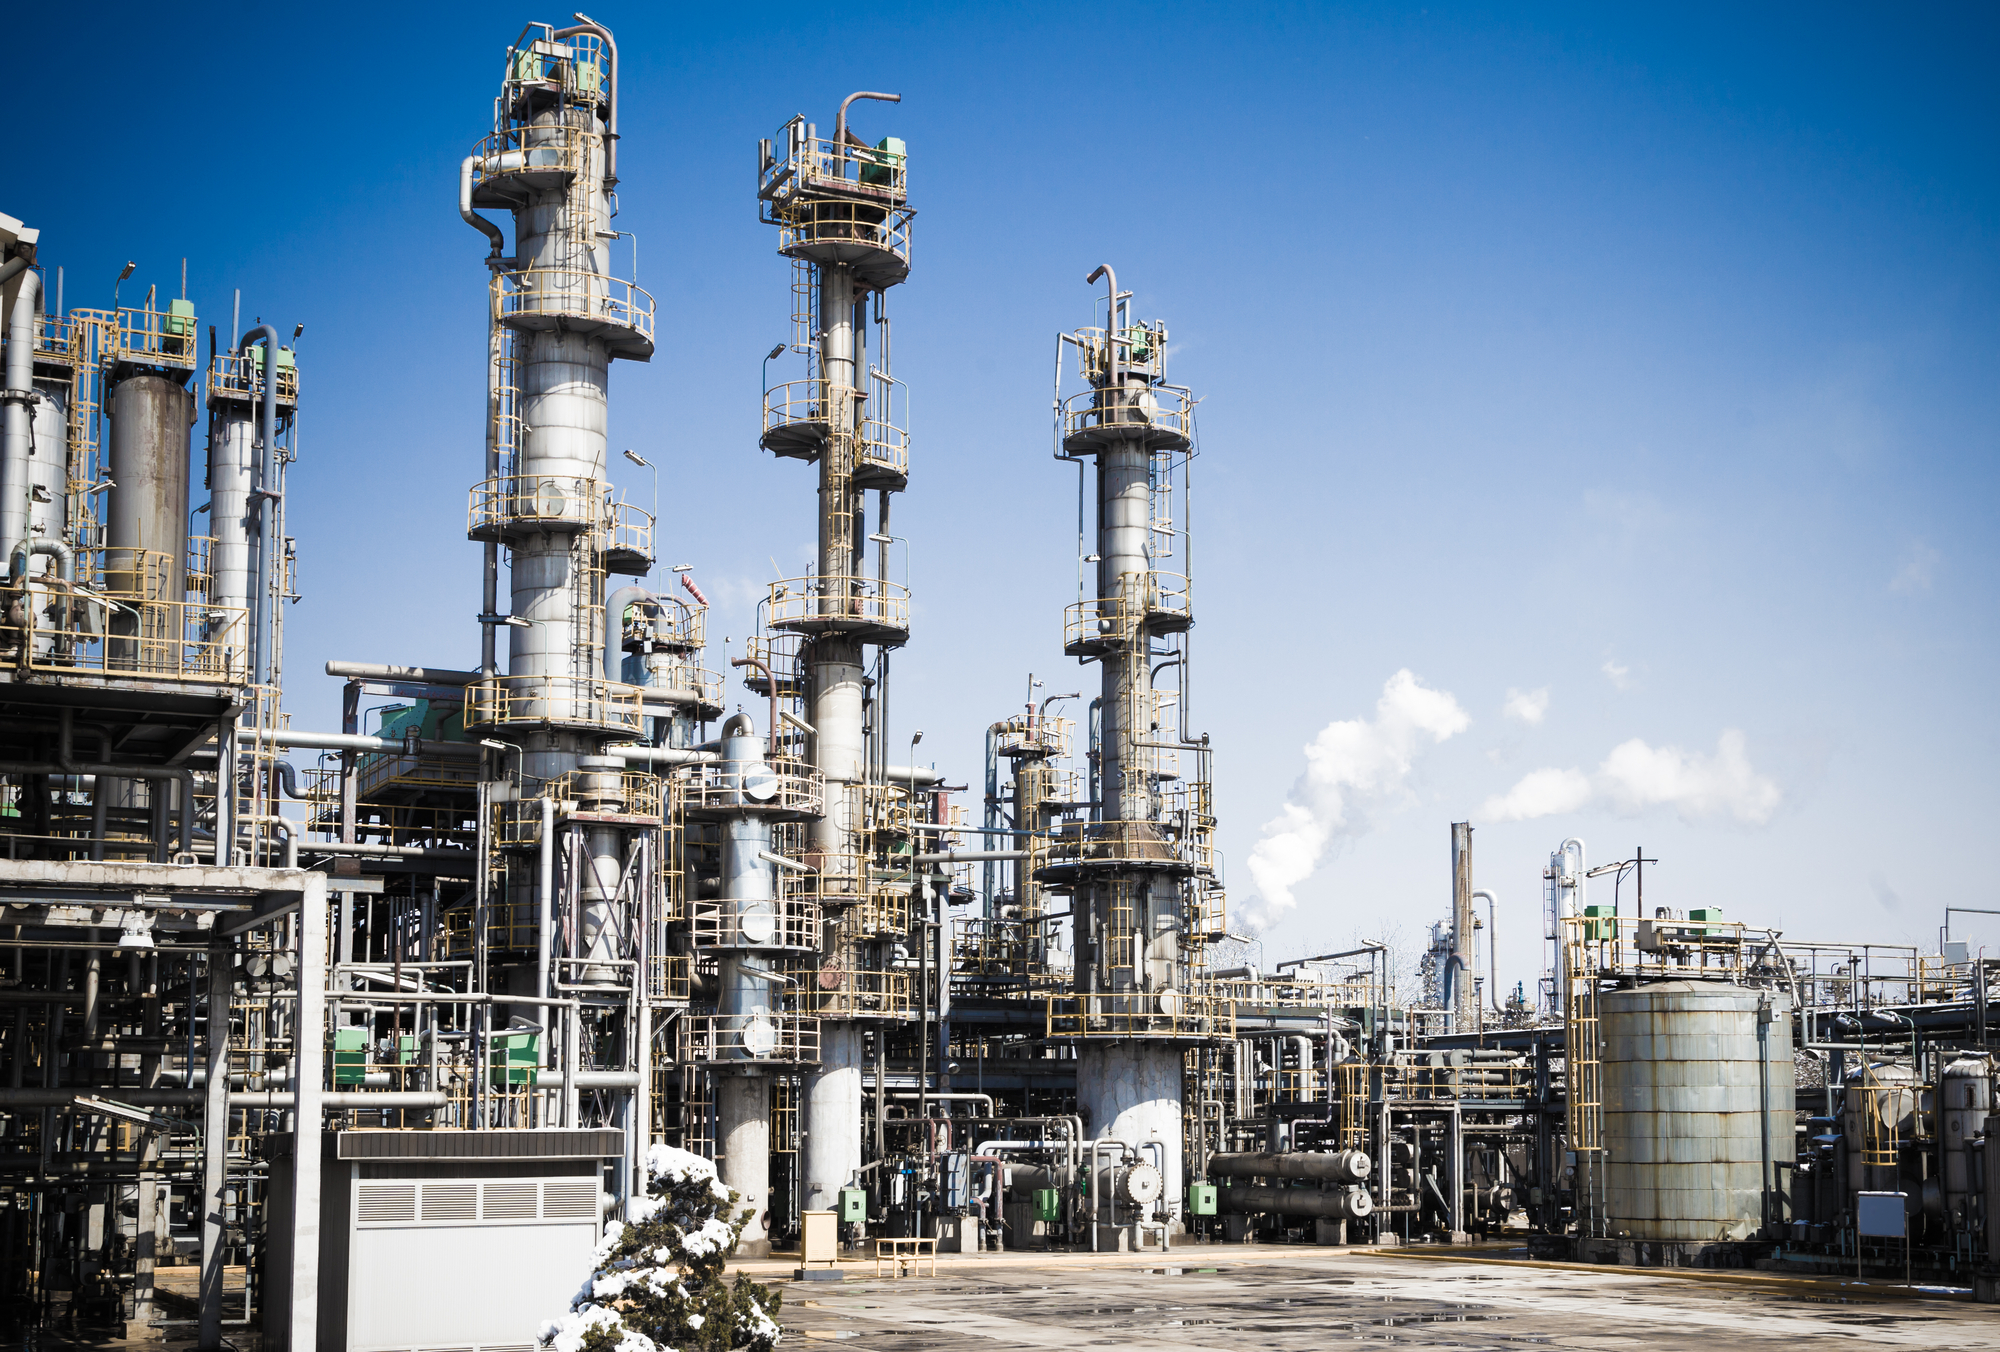
\includegraphics[width=\textwidth]{figs/column.jpg}
\caption{Distillation column.}
\label{fig:distillation column}
\end{figure}

The main goal of this research project is to investigate a batch
extractive distillation process using dimethyl sulfoxide as a solvent to
recover a distillate containing at least 99.75 mol\% isopropyl alcohol,
shortened to IPA in this document. This separation is especially
relevant to the pharmaceutical industry, where IPA is commonly used and
is often required in very high concentrations. The mixture to be
separated contains water, IPA, dimethyl sulfoxide, abbreviated as DMSO,
and a negligible amount of toluene. Simple batch distillation cannot be
used effectively for this regeneration process, since water and IPA form
a homogeneous minimum-boiling azeotrope at approximately 87--88 mass\%
IPA and 80.2--80.4 °C.

Furthermore, this project aims to analyze how operational and
geometrical parameters affect the performance of the distillation
process, how variations in the charge composition influence the
separation, and what column dimensions are required for efficient
operation. In addition to determining the optimal column height and
width, the study also examines different strategies for improving
solvent and material recovery, reducing waste, and increasing the
energetic efficiency of the process.

Extractive distillation involves the addition of a usually
low-volatility extra component to a mixture when separation by
conventional distillation is not possible. This additional component
increases the relative volatility difference between the components to
be separated, thereby allowing the azeotrope to be bypassed. It differs
from azeotropic distillation, in which the third component, often
referred to as an entrainer or extractive agent, forms a new low-boiling
azeotrope with one of the original components and is recovered from the
distillate rather than from the bottom of the column.

DMSO was selected as the solvent for this process because of its very
high boiling point, which is significantly greater than that of both
water and IPA. It is a stable, cost-effective, and highly effective
solvent with a strong affinity for water, while also being easily
recyclable. These properties make it suitable for extractive
distillation processes where high-purity IPA recovery is required.

For this project, ChemCAD modeling software was used to simulate the
batch extractive distillation process, predict phase compositions and
mixture behavior, obtain numerical data, and optimize the operating
conditions. Modeling is essential because it allows the separation
process to be evaluated and improved without the need to perform
numerous time-consuming laboratory experiments. Several ChemCAD
simulations were carried out to study not only the original separation
process, but also different recycling and energy-saving configurations.

Further simulations were conducted to investigate the possibility of
recycling IPA-water run-off material obtained from a previous
distillation. In one approach, this run-off material was added directly
to the new charge, while the remaining DMSO recovered from the previous
simulation was reused as the entrainer. In another approach, the
IPA-water run-off material was mixed with the DMSO-water run-off product
from the previous distillation, and the resulting mixture was added to
the new charge. These simulations were performed to evaluate whether
valuable material could be recovered and reused while maintaining the
required IPA purity in the distillate.

An additional simulation was also carried out in which the DMSO-water
run-off material was distilled separately in order to recover both the
entrainer and the water. The target purity for both recovered DMSO and
water was set at a minimum of 99.75 mol\%. This part of the study is
important for assessing the feasibility of solvent regeneration and
water reuse, both of which contribute to reducing waste and improving
the sustainability of the process.

Energy-saving alternatives were also investigated. One simulation
considered preheating the feed using vapor from the top of the
distillation column, with the aim of reducing the energy required to
heat the feed before separation. A further dynamic simulation was
performed in which the top vapor was compressed and its heat was used in
the reboiler to heat the charge. This configuration was studied as a
potential heat-integration strategy to decrease the overall energy
demand of the batch distillation operation.

In addition to the process simulations, the two main heat exchangers of
the system, namely the condenser and the reboiler, were designed. Their
main dimensions, number of tubes, wall thicknesses, and suitable
exchanger types were determined. Finally, a cost estimation was carried
out for the complete distillation column, including the main equipment
required for operation. This provides a broader technical and economic
evaluation of the proposed separation process.

Among the benefits of this distillation strategy are its versatility,
reduced waste generation, improved solvent recovery, scalability, and
potentially lower cost compared with alternative separation methods.
Since DMSO can be applied in a wide range of pharmaceutical processes
and enables the recovery of high-purity IPA from azeotropic mixtures,
the results of this study may provide a sustainable and industrially
relevant solution for handling IPA-water mixtures.

To summarize, the objectives of this project are the following:

\section{Objectives}\label{objectives}

\begin{itemize}
\tightlist
\item
  To propose the values of the geometrical and operational parameters of
  the batch extractive distillation process.
\item
  To study the influence of recycling the entrainer.
\item
  To study the influence of recycling the off-cuts.
\item
  To determine the main dimensions of the heat exchanger.
\item
  To study the possibility of heat recovery.
\end{itemize}

\newpage

\chapter{Theoretical Background}\label{theoretical-background}

\section{Batch Extractive
Distillation}\label{batch-extractive-distillation}

In batch extractive distillation, a mixture of a more volatile and a
less volatile component is cyclically heated and cooled to achieve the
component separation, by causing the more volatile component to
evaporate in a higher concentration and then condensate for its
recovery. This process is done in batch, where only a portion of the
mixture is treated in a single cycle; a fixed amount of it is to be
separated at a time {[}cite lecture{]}.

The distillate of the mixture is separated from the less volatile
substances that are left in the residue or at the bottom of the tanks,
by being brought back to its liquid phase by a condenser and then
collected. However, part of this condensate will return to the column as
reflux to improve the mass transfer between phases and therefore the
efficiency of the column, at a ratio we will call reflux ratio. It is
the quotient of the liquid used as reflux and the total liquid extracted
(distillate). The composition of our distillate will steadily change
(the more volatile component's mole fraction will decrease in the
distillate and increase the tank) as the procedure progresses
{[}cite{]}.

\begin{figure}[H]
\centering
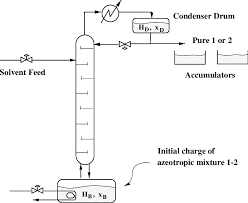
\includegraphics[width=0.4\textwidth]{figs/batchex.png}
\caption{A diagram illustrating batch extractive distillation.}
\label{fig:A diagram illustrating batch extractive distillation}
\end{figure}

\section{Azeotropes}\label{azeotropes}

Azeotropes can be described as a state of equilibrium reached by both
the liquid and gaseous phases inside the column, making the separation
of the initial mixture impossible. This is due to the fact that both
phases meet on the main diagonal line of the equilibrium curve diagram.
This would mean that x = y. This condition prevents any more separation
from happening, since the equilibrium reached eliminates the gradient
needed for further change in the concentrations {[}cite lecture{]}.

\begin{figure}[H]
\centering
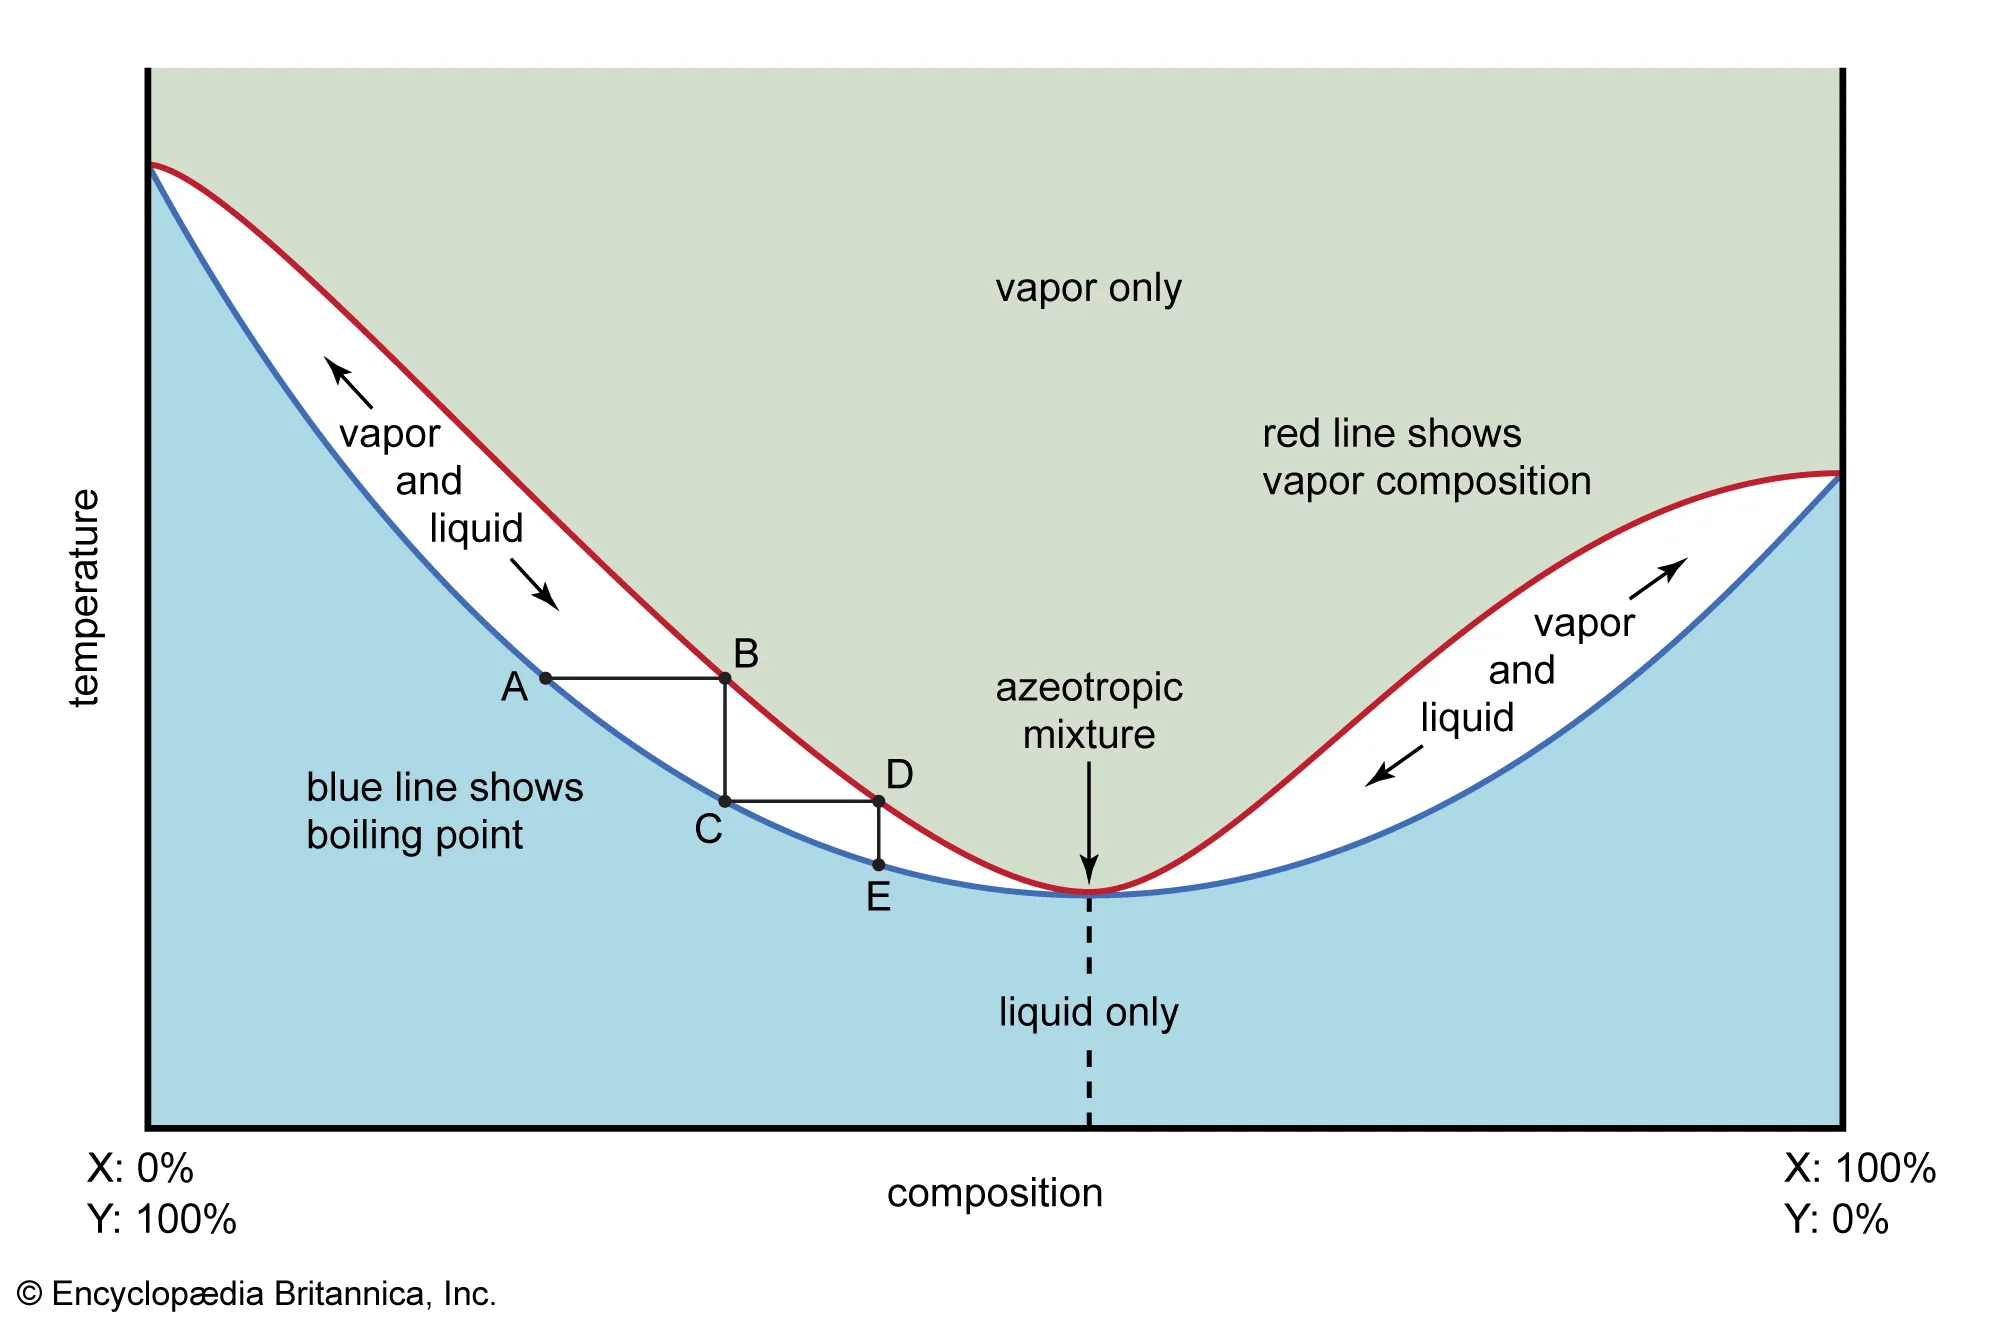
\includegraphics[width=0.8\textwidth]{figs/azeotropepic.png}
\caption{Visual representation of an azeotropic mixtureDiagram of the batch extractive distillation process.}
\label{fig:Visual representation of an azeotropic mixtureDiagram of the batch extractive distillation process}
\end{figure}

\section{Material Recovery in Extractive
Distillation}\label{material-recovery-in-extractive-distillation}

Material recovery is an important part of extractive distillation, since
the process requires the addition of a third component. The purpose of
this component is to change the relative volatility of the original
components and make the separation possible. However, because the
solvent is not the desired final product, it should be recovered and
reused whenever possible. This reduces the amount of fresh solvent
required, lowers operating costs, and decreases waste formation. In
extractive distillation, the solvent is usually chosen to have a much
higher boiling point than the components being separated, so it is
mostly recovered from the bottom product rather than from the
distillate. {[}Separation Process Principles by Seader, Henley, and
Roper{]}.

In batch extractive distillation, the recovery of materials is
especially relevant because the composition of the liquid in the still
pot changes continuously with time. As the operation progresses,
different fractions may be obtained: some fractions may meet the desired
purity specification, while others may contain valuable amounts of IPA,
water, or DMSO but not be pure enough to be considered final products.
These intermediate or run-off streams can often be recycled to a later
batch or treated in a separate recovery step.

For this project, material recovery is studied through the recycling of
run-off material and the recovery of DMSO from previous distillation
residues. Since DMSO acts as the extractive solvent, its recovery is
necessary for improving the economic and environmental performance of
the process. A separate recovery step can also be applied to DMSO-water
run-off material in order to obtain both water and DMSO at high purity.
Therefore, material recovery is not only a waste-reduction strategy, but
also an essential part of designing a sustainable extractive
distillation process.

\section{Heat Exchangers}\label{heat-exchangers}

Heat exchangers are devices used to transfer heat between two fluids at
different temperatures. In most industrial heat exchangers, the fluids
do not mix directly, but are separated by a solid wall through which
heat is transferred. The heat transfer process usually involves
convection from the hot fluid to the wall, conduction through the wall,
and convection from the wall to the cold fluid. Heat exchangers are
widely used in chemical and mechanical engineering for heating, cooling,
condensation, evaporation, and heat recovery. {[}Kern's Process Heat
Transfer{]}

In distillation systems, the two most important heat exchangers are the
condenser and the reboiler. The condenser removes heat from the vapor
leaving the top of the column and converts it into liquid. Part of this
liquid may be withdrawn as distillate, while the remaining part is
returned to the column as reflux. The reboiler, on the other hand,
supplies heat to the liquid at the bottom of the column, producing vapor
that rises through the column and allows mass transfer between vapor and
liquid phases.

The design of a heat exchanger depends mainly on the required heat duty,
the temperature difference between the fluids, the heat-transfer
coefficient, and the available heat-transfer area. A common design
equation is: \begin{equation}{Q = K A \Delta T_{lm} F}\end{equation}
where Q is the heat duty, k is the overall heat-transfer coefficient, A
is the heat-transfer area, ΔTlm is the logarithmic mean temperature
difference, and F is a correction factor. In this project, this theory
is applied to the design of the distillation column's condenser and
reboiler.

\begin{figure}[H]
\centering
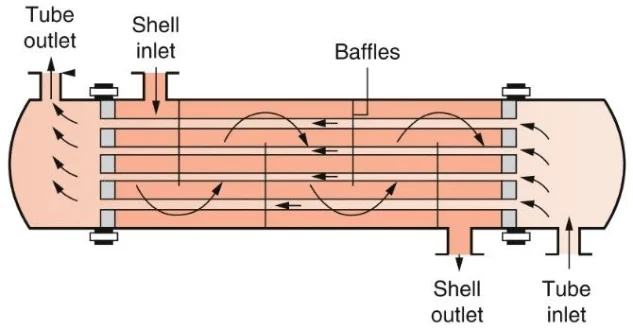
\includegraphics[width=0.8\textwidth]{figs/simpleshell.png}
\caption{Simple, single-pass shell and tube heat exchanger.}
\label{fig:Simple, single-pass shell and tube heat exchanger}
\end{figure}

\section{Heat Recycling in the
Industry}\label{heat-recycling-in-the-industry}

Heat recycling, also called heat recovery, is the reuse of heat that
would otherwise be rejected from a process. In many industrial systems,
some streams must be cooled while others must be heated. Instead of
using only external utilities, such as cooling water and steam, heat can
be transferred from hot process streams to cold process streams. This
reduces the energy demand of the plant and improves overall process
efficiency. {[}Kemp's Pinch Analysis and Process Integration{]}.

In distillation, heat recycling is especially important because the
process usually requires significant energy input in the reboiler and
significant heat removal in the condenser. One simple form of heat
recycling is feed preheating, where heat from a hot stream, such as
overhead vapor or bottom product, is used to increase the temperature of
the feed before it enters the column. This decreases the amount of heat
that must later be supplied by the reboiler.

A more advanced method is vapor recompression. In this method, the vapor
leaving the top of the column is compressed, which increases its
temperature and pressure. The compressed vapor can then be used as a
heating medium in the reboiler. Although the compressor requires
mechanical work, part of the heat that would normally be removed in the
condenser is reused. The goal is for the net output thermal energy of
the recycling system to be higher than the required input energy.

\chapter{Mixture Composition}\label{mixture-composition}

\section{Initial Conditions}\label{initial-conditions}

Our mixture to be separated has a volume of 3500 liters, and a
composition of 66.6 mol\% isopropanol, and 33.4 mol\% water. The time
available to complete the distillation process is 22 hours. Inside the
batch distillation column, the temperature will gradually increase until
it reaches the boiling point of the mixture, 80.2 ֯C. Our column was
assigned a number of theoretical stages n=12 (including the total
condenser and the still pot). The feed stage initially is the 5th
counted from the top. As for our entrainer, dimethyl sulfoxide (DMSO)
will be fed to the column at 100\% purity, room temperature (25 ֯C) and
1.013 bar in pressure. The chosen starting feed flow rate is 5 kmol/h.
These parameters are to be changed depending on the results.

\begin{longtable}[]{@{}
  >{\centering\arraybackslash}p{(\linewidth - 8\tabcolsep) * \real{0.1571}}
  >{\centering\arraybackslash}p{(\linewidth - 8\tabcolsep) * \real{0.2571}}
  >{\centering\arraybackslash}p{(\linewidth - 8\tabcolsep) * \real{0.1857}}
  >{\centering\arraybackslash}p{(\linewidth - 8\tabcolsep) * \real{0.1857}}
  >{\centering\arraybackslash}p{(\linewidth - 8\tabcolsep) * \real{0.2143}}@{}}
\caption{Binary interaction parameters.
\label{tab:Binary interaction parameters}}\tabularnewline
\toprule\noalign{}
\begin{minipage}[b]{\linewidth}\centering
I
\end{minipage} & \begin{minipage}[b]{\linewidth}\centering
J
\end{minipage} & \begin{minipage}[b]{\linewidth}\centering
Bij {[}Cal/mol{]}
\end{minipage} & \begin{minipage}[b]{\linewidth}\centering
Bji {[}Cal/mol{]}
\end{minipage} & \begin{minipage}[b]{\linewidth}\centering
Alpha {[}Cal/mol{]}
\end{minipage} \\
\midrule\noalign{}
\endfirsthead
\toprule\noalign{}
\begin{minipage}[b]{\linewidth}\centering
I
\end{minipage} & \begin{minipage}[b]{\linewidth}\centering
J
\end{minipage} & \begin{minipage}[b]{\linewidth}\centering
Bij {[}Cal/mol{]}
\end{minipage} & \begin{minipage}[b]{\linewidth}\centering
Bji {[}Cal/mol{]}
\end{minipage} & \begin{minipage}[b]{\linewidth}\centering
Alpha {[}Cal/mol{]}
\end{minipage} \\
\midrule\noalign{}
\endhead
\bottomrule\noalign{}
\endlastfoot
Isopropanol & Water & 20.0554 & 832.981 & 0.3255 \\
Isopropanol & Dimethyl Sulfoxide & 115.279 & -25.0123 & 0.4 \\
Water & Dimethyl Sulfoxide & 1203.77 & -524.822 & 0.6615 \\
\end{longtable}

In the table above we can find the binary interaction parameters (BIPs)
for our mixture, which are the coefficients to be used in the NRTL
thermodynamic model to describe the interactions between pairs of
molecules in our mixture. The BIPs describe the excess Gibbs free energy
of mixing\autocite{yao_ling_chien_2007}.

At the beginning of the process, we will start with total reflux (R=∞).
After the steady-state is reached, we will be working with an initial
reflux ratio of R=6, subject to change as the analysis progresses. In
the same manner, we will start with an initial feed temperature of 20°C,
12 stages, feed stage 4, and a feed flow rate of 5 kmol/h.

\section{Azeotrope Condition}\label{azeotrope-condition}

In our case, our azeotrope presents at a mass fraction of 87-88\% and a
temperature of 80.2 -- 80.4 °C. This is due to the interactions between
the molecules (see Table 1) of each component in the solution.

\begin{figure}[H]
\centering
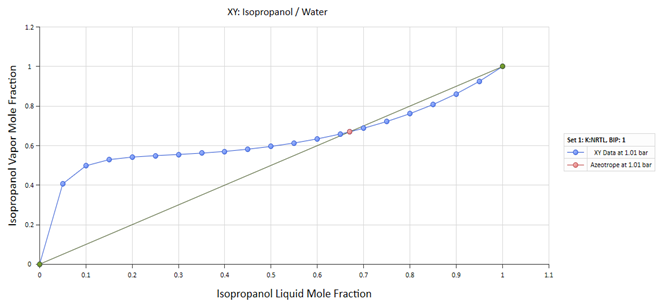
\includegraphics[width=0.9\textwidth]{figs/Picture1.png}
\caption{Graphical representation of the azeotrope present in the water/IPA mixture.}
\label{fig:Graphical representation of the azeotrope present in the water/IPA mixture}
\end{figure}

\section{Residue Curves}\label{residue-curves}

Our residue curves depict how the liquid composition in the distillation
still-pot evolves over time during simple batch distillation at 1.01
bar. Each vertex of the triangle represents 100\% of the component, and
for the IPA-water-DMSO system the curves start at the azeotrope, showing
the need for DMSO to carry out the separation. They, too, illustrate the
separation trajectory: the concentration of DMSO increases as time
progresses for every case, revealing that the distillation of this
mixture will generally lead to DMSO accumulation in the pot, while IPA
and water are removed. Similarly, the diagram tells us that DMSO forms
no azeotropes with the other two components.

\begin{figure}[H]
\centering
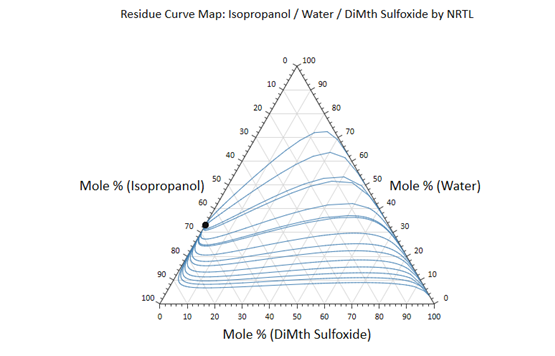
\includegraphics[width=0.8\textwidth]{figs/Picture2.png}
\caption{Residue curves of our mixture.}
\label{fig:Residue curves of our mixture.}
\end{figure}

\chapter{Parameter Effects}\label{parameter-effects}

\section{Targets}\label{targets}

For the dehydration of isopropanol, the distillate's solution must be ≥
99.75 mol\% IPA, ≤ 0.55 mol\% water, and ≤ 0.15 mol\% dimethyl
sulfoxide. At the time of recovery, the water will be extracted as
distillate. In this solution, less than 0.05 mol\% IPA should be
present, and less than 0.035 mol\% DMSO. After the whole process is
finished, we will collect the remaining DMSO from the bottom of the
column; We will use the same purity requirements stated for IPA, that
is, ≥ 99.75 mol\% DMSO, ≤ 0.55 mol\% water, and ≤ 0.15 mol\% IPA.

\section{Parameters studied}\label{parameters-studied}

\begin{itemize}
\tightlist
\item
  Feed stage {[}-{]}
\item
  Reflux ratio {[}-{]}
\item
  Number of stages {[}-{]}
\item
  Feed flow rate {[}kmol/h{]}
\item
  Feed Temperature {[}°C{]}
\end{itemize}

Dependable variables:

\begin{itemize}
\tightlist
\item
  Mass of the IPA product
\item
  Time
\item
  Molar fraction (purity) of the product
\end{itemize}

Goals:

\begin{itemize}
\tightlist
\item
  Maximum mass
\item
  Minimum time
\item
  Maximum purity distillate (≥0.975 mole fraction IPA, ≤0.0025 water,
  ≤0.0015 DMSO)
\end{itemize}

Constant values:

\begin{itemize}
\tightlist
\item
  Volume of charge: 3500 dm3
\item
  Charge temperature: 80֯C
\item
  Reboiler duty: 1000 MJ/h
\item
  Charge composition:

  \begin{itemize}
  \tightlist
  \item
    0.66 mole fraction IPA
  \item
    0.34 mole fraction water
  \end{itemize}
\item
  Feed composition: 1 mole fraction DMSO (theoretically)
\end{itemize}

We have adhered to an interval of 15-30 for the number of stages, 5-10
kmol/h for the feed rate, 4-8 for the feed stage, 50-70 °C for the feed
temperature, and 4-6 for the reflux ratio, as these are common
industrial values that have showed good efficiency of separation in
literature {[}cite{]}. A quite difficult, azeotropic separation calls
for many stages and a high R.

It is worth mentioning that, in simulations where the feed temperature
is not being evaluated, a constant feed temperature value of 70֯C is
chosen. All parameters were studied in the order in which they will be
presented below. For parameters besides feed temperature, their constant
values during the initial simulations were the averaged value of the
ranges mentioned previously (22 stages, a feed rate of 7.5 kmol/h, a
feed in stage number 6, and a reflux ratio of 5).

Below, we can see the purity results and total elapsed time of the last
attempts tried with different parameter values; data obtained from
sensitivity analyses. The final parameters were chosen through an
iterative process, in which a sensitivity analysis is conducted,
parameters were changed to achieve optimal results, and another
sensitivity analysis is carried out until results are satisfactory.

\begin{longtable}[]{@{}rrrrr@{}}
\caption{Feed Stage Data\\
\label{tab:Feed Stage Data}}\tabularnewline
\toprule\noalign{}
Trial & Feed Stage & Mole Fraction & Time (h) & Mass (kg) \\
\midrule\noalign{}
\endfirsthead
\toprule\noalign{}
Trial & Feed Stage & Mole Fraction & Time (h) & Mass (kg) \\
\midrule\noalign{}
\endhead
\bottomrule\noalign{}
\endlastfoot
1 & 1 & 0.727319 & 8.45001 & 3509.90 \\
2 & 3.66667 & 0.997528 & 9.20002 & 2380.31 \\
3 & 6.33333 & 0.997400 & 9.20002 & 2381.18 \\
4 & 9 & 0.997040 & 9.20002 & 2380.57 \\
5 & 11.6667 & 0.997273 & 9.15002 & 2370.28 \\
6 & 14.3333 & 0.995347 & 8.50001 & 2225.38 \\
7 & 17 & 0.986126 & 8.15001 & 2132.24 \\
8 & 19.6667 & 0.970703 & 7.90001 & 2051.91 \\
9 & 22.3333 & 0.904141 & 8.20001 & 2021.87 \\
10 & 25 & 0.717659 & 13.55 & 2696.94 \\
\end{longtable}

Which can be plotted as:

\begin{figure}[H]
\centering

    \begin{subfigure}{0.48\textwidth}
        \centering
        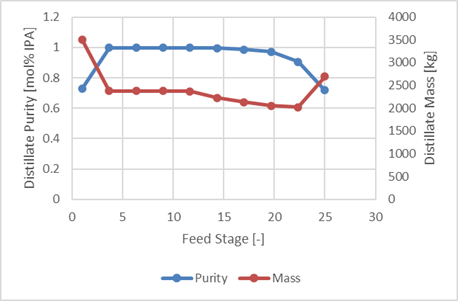
\includegraphics[width=\textwidth]{figs/feedstagepuritymass.png}
    \end{subfigure}
    \hfill
    \begin{subfigure}{0.48\textwidth}
        \centering
        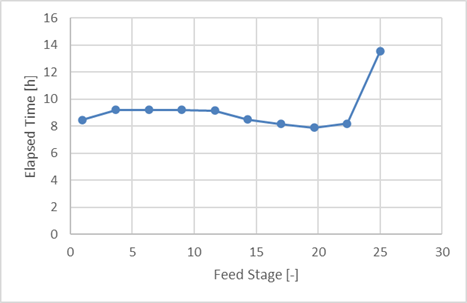
\includegraphics[width=\textwidth]{figs/feedstagetime.png}
    \end{subfigure}

    \caption{Feed stage effect on purity, mass and time.}
    \label{fig:Feed stage effect on purity, mass}

\end{figure}

\begin{longtable}[]{@{}rrrrr@{}}
\caption{Reflux Ratio Data\\
\label{tab:Reflux Ratio Data}}\tabularnewline
\toprule\noalign{}
Trial & Reflux Ratio & Mole Fraction & Time (h) & Mass (kg) \\
\midrule\noalign{}
\endfirsthead
\toprule\noalign{}
Trial & Reflux Ratio & Mole Fraction & Time (h) & Mass (kg) \\
\midrule\noalign{}
\endhead
\bottomrule\noalign{}
\endlastfoot
1 & 3 & 0.996872 & 16.15 & 2393.41 \\
2 & 4 & 0.997535 & 18.05 & 2406.52 \\
3 & 5 & 0.997973 & 19.95 & 2413.92 \\
4 & 6 & 0.997399 & 21.90 & 2424.64 \\
5 & 7 & 0.997836 & 23.7999 & 2426.82 \\
\end{longtable}

Which can be plotted as:

\begin{figure}[H]
\centering

    \begin{subfigure}{0.48\textwidth}
        \centering
        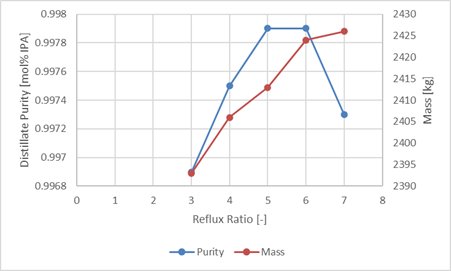
\includegraphics[width=\textwidth]{figs/Rpuritymass.png}
    \end{subfigure}
    \hfill
    \begin{subfigure}{0.48\textwidth}
        \centering
        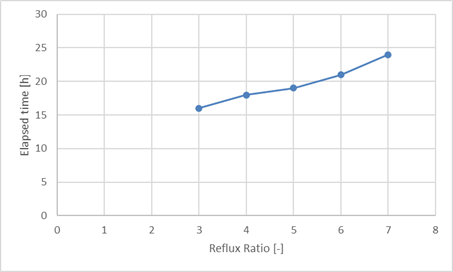
\includegraphics[width=\textwidth]{figs/Rtime.png}
    \end{subfigure}

    \caption{Reflux ratio effect on purity, mass and time.}
    \label{fig:Reflux ratio effect on purity, mass and time}

\end{figure}

\begin{longtable}[]{@{}rrrrr@{}}
\caption{Feed Rate Data\\
\label{tab:Feed Rate Data}}\tabularnewline
\toprule\noalign{}
Trial & Feed Rate (kmol/h) & Mole Fraction & Time (h) & Mass (kg) \\
\midrule\noalign{}
\endfirsthead
\toprule\noalign{}
Trial & Feed Rate (kmol/h) & Mole Fraction & Time (h) & Mass (kg) \\
\midrule\noalign{}
\endhead
\bottomrule\noalign{}
\endlastfoot
1 & 5 & 0.987313 & 8.60001 & 2375.32 \\
2 & 6.11111 & 0.995814 & 8.65001 & 2356.56 \\
3 & 7.22222 & 0.997105 & 8.95002 & 2381.33 \\
4 & 8.33334 & 0.996503 & 9.20002 & 2387.23 \\
5 & 9.44445 & 0.997112 & 9.40002 & 2380.46 \\
6 & 10.5556 & 0.996768 & 9.65002 & 2379.43 \\
7 & 11.6667 & 0.996776 & 9.90002 & 2375.50 \\
8 & 12.7778 & 0.997171 & 10.15 & 2368.91 \\
9 & 13.8889 & 0.996996 & 10.45 & 2367.03 \\
10 & 15 & 0.997244 & 10.75 & 2362.07 \\
\end{longtable}

Which can be plotted as:

\begin{figure}[H]
\centering

    \begin{subfigure}{0.48\textwidth}
        \centering
        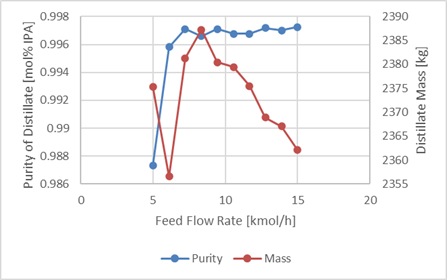
\includegraphics[width=\textwidth]{figs/feedratepuritymass.png}
    \end{subfigure}
    \hfill
    \begin{subfigure}{0.48\textwidth}
        \centering
        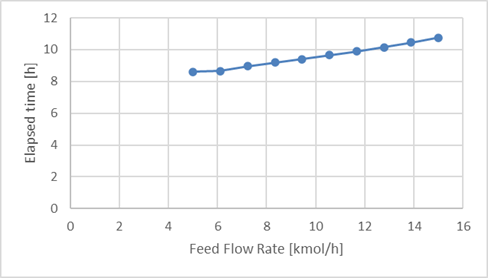
\includegraphics[width=\textwidth]{figs/feedratetime.png}
    \end{subfigure}

    \caption{Feed rate effect on purity, mass and time.}
    \label{fig:Feed rate effect on purity, mass and time}

\end{figure}

\begin{longtable}[]{@{}rrrrr@{}}
\caption{Stage Number Data\\
\label{tab:Stage Number Data}}\tabularnewline
\toprule\noalign{}
Trial & Stage Number & Mole Fraction & Time (h) & Mass (kg) \\
\midrule\noalign{}
\endfirsthead
\toprule\noalign{}
Trial & Stage Number & Mole Fraction & Time (h) & Mass (kg) \\
\midrule\noalign{}
\endhead
\bottomrule\noalign{}
\endlastfoot
1 & 10 & 0.907955 & 8.15001 & 2016.42 \\
2 & 12.2222 & 0.958189 & 7.85001 & 2022.11 \\
3 & 14.4444 & 0.980373 & 8.05001 & 2100.75 \\
4 & 16.6667 & 0.990602 & 8.30001 & 2173.13 \\
5 & 18.8889 & 0.995448 & 8.50001 & 2225.54 \\
6 & 21.1111 & 0.997299 & 9.15002 & 2370.32 \\
7 & 23.3333 & 0.997048 & 9.20002 & 2380.59 \\
8 & 25.5556 & 0.997349 & 9.20002 & 2381.05 \\
9 & 27.7778 & 0.997496 & 9.20002 & 2381.28 \\
10 & 30 & 0.997590 & 9.20002 & 2381.42 \\
\end{longtable}

Which can be plotted as:

\begin{figure}[H]
\centering

    \begin{subfigure}{0.48\textwidth}
        \centering
        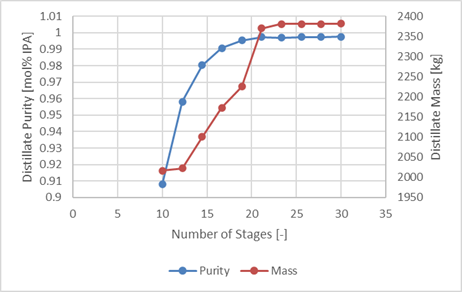
\includegraphics[width=\textwidth]{figs/stageNpuritymass.png}
    \end{subfigure}
    \hfill
    \begin{subfigure}{0.48\textwidth}
        \centering
        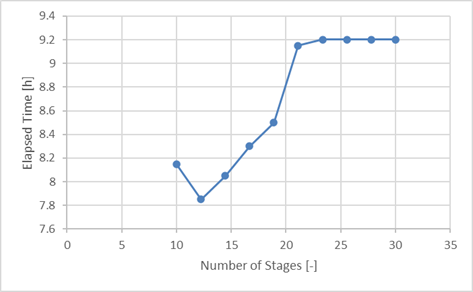
\includegraphics[width=\textwidth]{figs/stageNtime.png}
    \end{subfigure}

    \caption{Stage number effect on purity, mass and time.}
    \label{fig:Stage number effect on purity, mass and time}

\end{figure}

\begin{longtable}[]{@{}rrrrr@{}}
\caption{Feed Temperature Data\\
\label{tab:Feed Temperature Data}}\tabularnewline
\toprule\noalign{}
Trial & Feed Temperature (°C) & Mole Fraction & Time (h) & Mass (kg) \\
\midrule\noalign{}
\endfirsthead
\toprule\noalign{}
Trial & Feed Temperature (°C) & Mole Fraction & Time (h) & Mass (kg) \\
\midrule\noalign{}
\endhead
\bottomrule\noalign{}
\endlastfoot
1 & 20 & 0.996916 & 9.90002 & 2391.57 \\
2 & 32 & 0.996842 & 9.70002 & 2390.15 \\
3 & 44 & 0.996943 & 9.50002 & 2387.46 \\
4 & 56 & 0.997194 & 9.30002 & 2383.51 \\
5 & 68 & 0.997534 & 9.10002 & 2378.27 \\
6 & 80 & 0.996955 & 8.95002 & 2381.23 \\
\end{longtable}

Which can be plotted as:

\begin{figure}[H]
\centering

    \begin{subfigure}{0.48\textwidth}
        \centering
        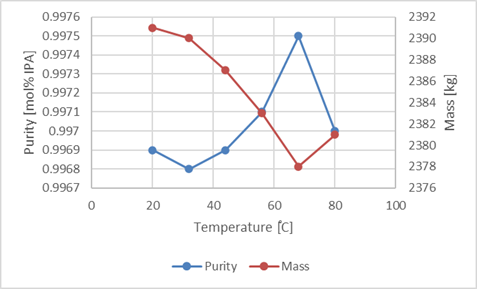
\includegraphics[width=\textwidth]{figs/feedTpuritymass.png}
    \end{subfigure}
    \hfill
    \begin{subfigure}{0.48\textwidth}
        \centering
        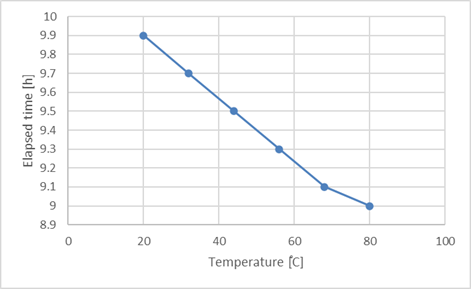
\includegraphics[width=\textwidth]{figs/feedTtime.png}
    \end{subfigure}

    \caption{Feed temperature effect on purity, mass and time.}
    \label{fig:Feed temperature effect on purity, mass and time}

\end{figure}

\section{Conclusion on Parameter
Effects}\label{conclusion-on-parameter-effects}

The sensitivity analyses show that each parameter affects the IPA
distillate purity, recovered mass, and elapsed time through different
mechanisms. The feed stage strongly influences the contact between the
DMSO feed and the internal vapour-liquid flows. If the feed is
introduced too high, the solvent does not interact sufficiently with the
liquid phase; if it is introduced too low, it cannot modify the relative
volatility across enough of the column. For this reason, the best
results occur at intermediate feed stages, while the extremes show clear
drops in purity and, in one case, a strong increase in time. The reflux
ratio improves separation by returning more condensed liquid to the
column, increasing vapour-liquid contact. However, after a certain
point, higher reflux gives only small purity improvements while greatly
increasing the operating time, so the purity peak at the middle reflux
values is more useful than simply choosing the highest reflux ratio. The
feed flow rate mainly controls how much DMSO is available to break the
IPA-water azeotropic behavior. Too low a flow rate gives insufficient
solvent action, while too high a flow rate increases the elapsed time
and can slightly reduce the recovered mass; therefore, an intermediate
feed rate is preferred. Increasing the number of stages improves purity
and mass because more equilibrium contacts are available, but the effect
reaches a plateau at higher stage numbers, meaning that additional
stages give diminishing returns and would mainly increase column size
and cost. Finally, increasing feed temperature reduces the elapsed time
because the feed enters closer to column conditions, but excessive
heating can disturb the internal temperature and composition profiles.
The purity peak occurs at a moderately high feed temperature, while the
recovered mass tends to decrease as temperature rises. Overall, the
selected parameter values should represent a compromise between high
purity, high recovered mass, and low elapsed time, rather than the
maximum value of only one dependent variable.

\begin{longtable}[]{@{}
  >{\centering\arraybackslash}p{(\linewidth - 8\tabcolsep) * \real{0.1471}}
  >{\centering\arraybackslash}p{(\linewidth - 8\tabcolsep) * \real{0.1765}}
  >{\centering\arraybackslash}p{(\linewidth - 8\tabcolsep) * \real{0.2059}}
  >{\centering\arraybackslash}p{(\linewidth - 8\tabcolsep) * \real{0.2353}}
  >{\centering\arraybackslash}p{(\linewidth - 8\tabcolsep) * \real{0.2353}}@{}}
\caption{Selected parameter values.
\label{tab:Selected parameter values}}\tabularnewline
\toprule\noalign{}
\begin{minipage}[b]{\linewidth}\centering
Feed Stage
\end{minipage} & \begin{minipage}[b]{\linewidth}\centering
Reflux Ratio
\end{minipage} & \begin{minipage}[b]{\linewidth}\centering
Feed Flow Rate
\end{minipage} & \begin{minipage}[b]{\linewidth}\centering
Number of Stages
\end{minipage} & \begin{minipage}[b]{\linewidth}\centering
Feed Temperature
\end{minipage} \\
\midrule\noalign{}
\endfirsthead
\toprule\noalign{}
\begin{minipage}[b]{\linewidth}\centering
Feed Stage
\end{minipage} & \begin{minipage}[b]{\linewidth}\centering
Reflux Ratio
\end{minipage} & \begin{minipage}[b]{\linewidth}\centering
Feed Flow Rate
\end{minipage} & \begin{minipage}[b]{\linewidth}\centering
Number of Stages
\end{minipage} & \begin{minipage}[b]{\linewidth}\centering
Feed Temperature
\end{minipage} \\
\midrule\noalign{}
\endhead
\bottomrule\noalign{}
\endlastfoot
4 & 4 & 7.5 kmol/h & 24 & 62 °C \\
\end{longtable}

These final parameters were chosen taking maximum efficiency into
consideration; they produce the best, balanced results regarding purity,
elapsed time and mass. We selected 24 stages for our column because,
even though the elapsed time is high, it will give us the best purity
results and the most amount of mass. A feed stage of 4 gives us a good
balance between distillate purity and mass, while keeping time at a
minimum. A feed stage higher than 22 will give us good purity results
too, but it will increase the time significantly. As for the selected
feed flow rate, a value between 6 and 7 kmol/h will be best, since we
are able to complete the process at the shortest possible time and
obtain the maximum amount of mass, with highest purity. Therefore, we
have settled on 7.5 kmol/h, or 586.012 kg/h. A reflux ratio of 6 would
give us the best results according to our graph; however, the time a
high reflux ratio needs and the energy it consumes are significantly
higher. A reflux ratio of 4 gives us good enough results, while making
up for time. Feed temperature is chosen to be 62°C because, even though
we won't obtain the highest amount of distillate possible, it will
reduce our elapsed time and give us the highest possible IPA purity.

\chapter{Effects of the charge
composition}\label{effects-of-the-charge-composition}

In this chapter, we will evaluate the effects that different charge
compositions have on the IPA distillate purity, the distillation time,
and the IPA recovery.

To do this, besides the original one, we will choose five different
charge compositions from which to calculate with:

\begin{itemize}
\tightlist
\item
  10 mol\% IPA in the charge mixture
\item
  30 mol\% IPA in the charge mixture
\item
  50 mol\% IPA in the charge mixture
\item
  75 mol\% IPA in the charge mixture
\item
  90 mol\% IPA in the charge mixture
\end{itemize}

We will observe the reflected effects of these mixtures in regards to:

\begin{itemize}
\tightlist
\item
  Efficiency
\item
  Elapsed time
\end{itemize}

From which, efficiency was calculated with the following formula:

\(\eta =\frac{n_{\mathrm{IPA,distillate}} \cdot x_{\mathrm{IPA,charge}}}{n_{\mathrm{IPA,charge}} \cdot x_{\mathrm{IPA,distillate}}}\cdot 100\)

\begin{itemize}
\tightlist
\item
  \(\eta\) = IPA recovery efficiency, in \%
\item
  \(n_{\mathrm{IPA,distillate}}\) = amount of IPA recovered in the
  distillate, in mol or kmol
\item
  \(n_{\mathrm{IPA,charge}}\) = amount of IPA initially present in the
  charge, in mol or kmol
\item
  \(x_{\mathrm{IPA,charge}}\) = IPA mole fraction in the initial charge
\item
  \(x_{\mathrm{IPA,distillate}}\) = IPA mole fraction in the recovered
  distillate
\end{itemize}

After changing the charge mixture to the above compositions, the
following results were obtained:

\begin{figure}[H]
\centering
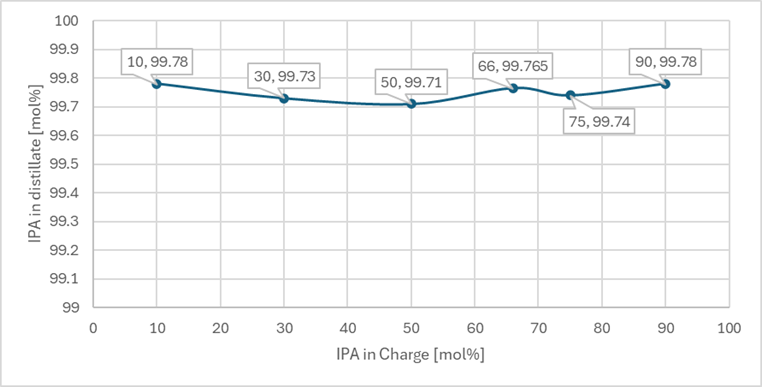
\includegraphics[width=0.6\textwidth]{figs/charge.png}
\caption{IPA mol\% in distillate as a function of IPA mol\% in charge.}
\label{fig:ipa-distillate-vs-charge}
\end{figure}

\begin{figure}[H]
\centering
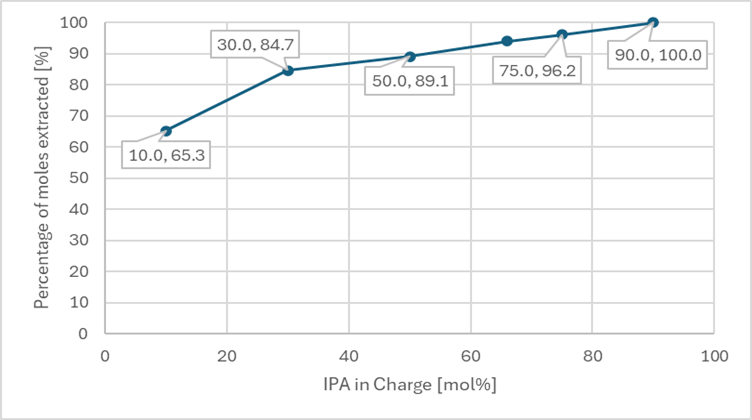
\includegraphics[width=0.6\textwidth]{figs/charge_3.png}
\caption{Efficiency $\eta$ as a function of IPA mol\% in charge.}
\label{fig:efficiency-vs-charge}
\end{figure}

\begin{figure}[H]
\centering
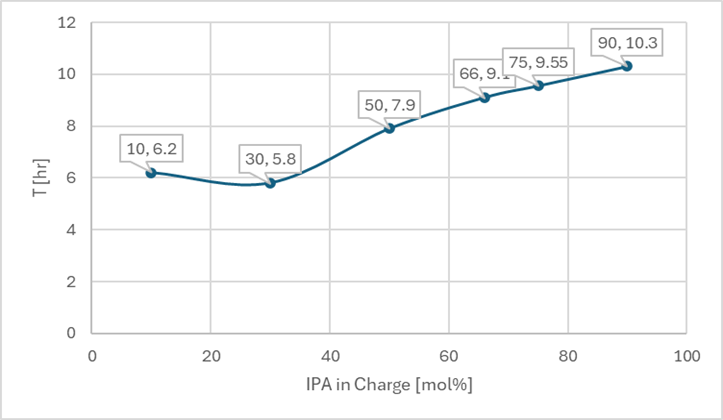
\includegraphics[width=0.6\textwidth]{figs/charge_2.png}
\caption{Elapsed time as a function of IPA mol\% in charge.}
\label{fig:elapsed-time-vs-charge}
\end{figure}

We can observe that, as the percentage of IPA in the charge increases,
it gets easier to extract and therefore, the efficiency is higher;
however, time also increases when the amount of IPA makes up most of the
mixture (≥50\%). It can be concluded that distillate purity is not
strongly dependent on charge composition, but rather, the elapsed time
is.

\chapter{Distillation Results}\label{distillation-results}

\section{Purity, Mass and Elapsed
Time}\label{purity-mass-and-elapsed-time}

We achieved a maximum purity of 99.856 mol\% IPA, meeting our
requirements; 0.14 ≤ 0.25 mol\% water, 0.0012 ≤0.15 mol\% DMSO. The
total elapsed time was 9.05 hours.

\begin{figure}[H]
\centering
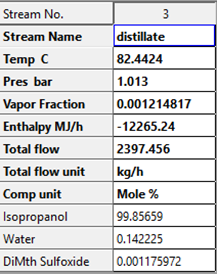
\includegraphics[width=0.4\textwidth]{figs/Picture20.png}
\caption{Stream results.}
\label{fig:Stream results}
\end{figure}

\section{Distillate Graph}\label{distillate-graph}

From the graphs produced by the ChemCAD simulation, it is possible to
observe how the composition of the distillate changed with time, under
our chosen parameter values:

\begin{figure}[H]
\centering
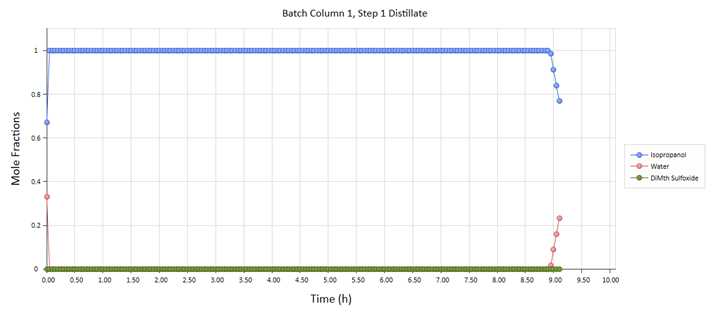
\includegraphics[width=\textwidth]{figs/Picture21.png}
\caption{Depiction of the distillate composition’s change with time.}
\label{fig:Depiction of the distillate composition’s change with time}
\end{figure}

The distillate composition graph shows that the IPA mole fraction
remains very high during most of the main distillation step, while the
water and DMSO mole fractions remain low. This confirms that the
selected operating parameters allow IPA to be removed as the main
overhead product with only small amounts of impurities. Near the end of
the step, the IPA mole fraction begins to decrease while the impurity
content increases, indicating that the useful IPA-rich distillation
period is ending. Therefore, the stopping point was selected before a
significant decrease in distillate purity occurs, in order to maintain
the required product specification.

\section{Effect on the Azeotrope}\label{effect-on-the-azeotrope}

The altered activity coefficients increase IPA's relative volatility
compared to water. This shifts the VLE curve, eliminating the original
azeotropic point where x = y. DMSO's high boiling point (189°C) ensures
it mostly remains in the liquid phase, accumulating in the column's
stripping section. This prevents IPA-water azeotrope reformation and
allows IPA to distill overhead. As we can see in graphs 14-17, The
IPA-water-DMSO system no longer exhibits an azeotrope, enabling
distillation to achieve \textgreater99.75\% IPA purity.

\begin{figure}[H]
\centering

    \begin{subfigure}{0.48\textwidth}
        \centering
        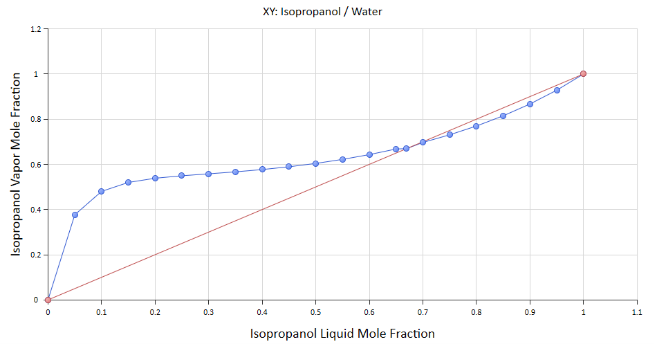
\includegraphics[width=\textwidth]{figs/Picture22.png}
    \end{subfigure}
    \hfill
    \begin{subfigure}{0.48\textwidth}
        \centering
        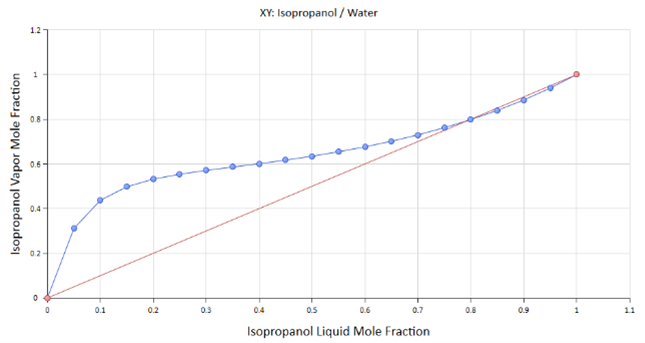
\includegraphics[width=\textwidth]{figs/Picture23.png}
    \end{subfigure}

    \par\medskip

    \begin{subfigure}{0.48\textwidth}
        \centering
        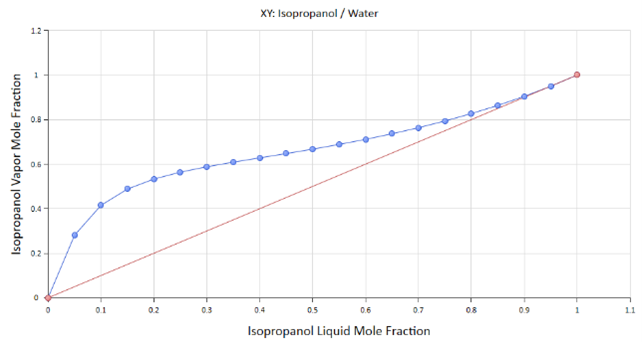
\includegraphics[width=\textwidth]{figs/Picture24.png}
    \end{subfigure}
    \hfill
    \begin{subfigure}{0.48\textwidth}
        \centering
        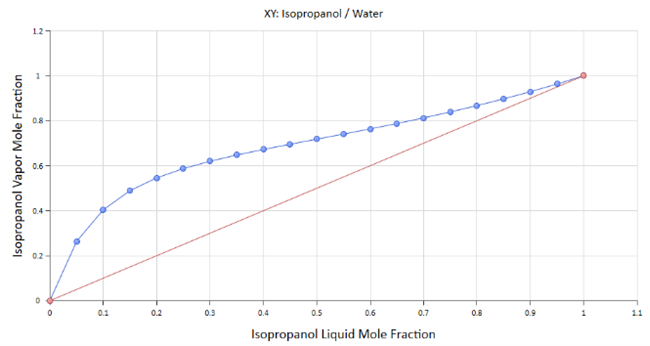
\includegraphics[width=\textwidth]{figs/Picture25.png}
    \end{subfigure}

    \caption{Effect the DMSO concentration (at 0.01, 0.05, 0.1 and 0.2 mole fraction, respectively) in the charge composition has on the azeotrope.}
    \label{fig:Effect the DMSO concentration in the charge composition has on the azeotrope}

\end{figure}

The VLE diagrams show that the addition of DMSO changes the
phase-equilibrium behavior of the IPA-water system. Without entrainer,
the IPA-water mixture forms an azeotrope, which limits the maximum IPA
purity attainable by ordinary distillation. When DMSO is added, the
equilibrium curve is shifted away from the diagonal, meaning that the
vapour and liquid compositions are no longer equal at the original
azeotropic point. This confirms that DMSO successfully changes the
relative volatility of IPA and water, allowing IPA to be concentrated
beyond the azeotropic composition. The effect becomes more visible as
the DMSO mole fraction increases, showing that the entrainer is
essential for achieving the required high-purity IPA distillate.

\section{Additional Stages}\label{additional-stages}

After obtaining our desired product, the distillation column will still
have liquid at the bottom, which composition is still rich in all three
components: water, DMSO and IPA.

In an attempt to recover as much water as possible, as well as solvent,
three more stages to the process were added: a water-IPA run-off stage,
a water distillation stage, and a water-DMSO run-off stage.

In the water-IPA run-off stage, we will attempt to dispose of all
leftover IPA in the bottom, in order to extract water more efficiently
in the next phase. In the water distillation stage, we will separate as
much water from the leftover mixture as possible, with the same purity
parameters as IPA.Finally, for the water-DMSO run-off stage, we want to
leave as little water in the bottom as possible in order to recover the
solvent, again, following the same purity requirements as IPA.

In this case, extensive sensitivity analyses were not carried out, since
our investigated parameters were now set to the chosen values for the
whole process. Instead, the stop values for each stage were set as the
following:

\begin{itemize}
\tightlist
\item
  stop value for step 2: 0.8 mole fraction water in the accumulator
\item
  stop value for step 3: 0.9995 mole fraction water in the accumulator
\item
  stop value for step 4: 0.9995 mole fraction DMSO in the bottom tank
\end{itemize}

The stop values were chosen according to the purpose of each additional
distillation step. In step 2, the objective is not to obtain a final
pure product, but to remove the remaining IPA-rich fraction before the
main water recovery step. Therefore, the step is stopped when the
accumulator reaches a high water content, indicating that most of the
remaining IPA has already been removed from the bottom mixture. In step
3, the goal is to recover water as a final product, so a much stricter
stop value is used: the accumulator must reach approximately pure water.
In step 4, the objective is to recover the DMSO remaining in the bottom
tank, so the process is continued until the bottom product reaches the
required DMSO purity.

And our chosen reflux ratio for each step were chosen in a small
iteration process, using values ranging from 2 to 5 R {[}cite source{]}.
After 4 iterations were carried out for each step, the following values
yielded the best results in the least possible amount of time:

\begin{itemize}
\tightlist
\item
  R for step 2: 5
\item
  R for step 3: 4
\item
  R for step 4: 2
\end{itemize}

A higher reflux ratio was used in step 2 because this step handles a
transition mixture containing IPA and water, and stronger internal
liquid-vapour contact is needed to remove the remaining IPA effectively.
Step 3 uses a moderate reflux ratio because water is the main volatile
component and can be recovered at high purity without excessive reflux.
Step 4 uses the lowest reflux ratio because the target product is the
DMSO-rich bottom stream rather than the distillate; therefore, very high
reflux is not necessary and would only increase the operating time.

This will allow us to carry out our simulation until our desired
purities for both water and DMSO are reached.

The resulting graphs of the additional distillation stages are showcased
below:

\begin{figure}[H]
\centering
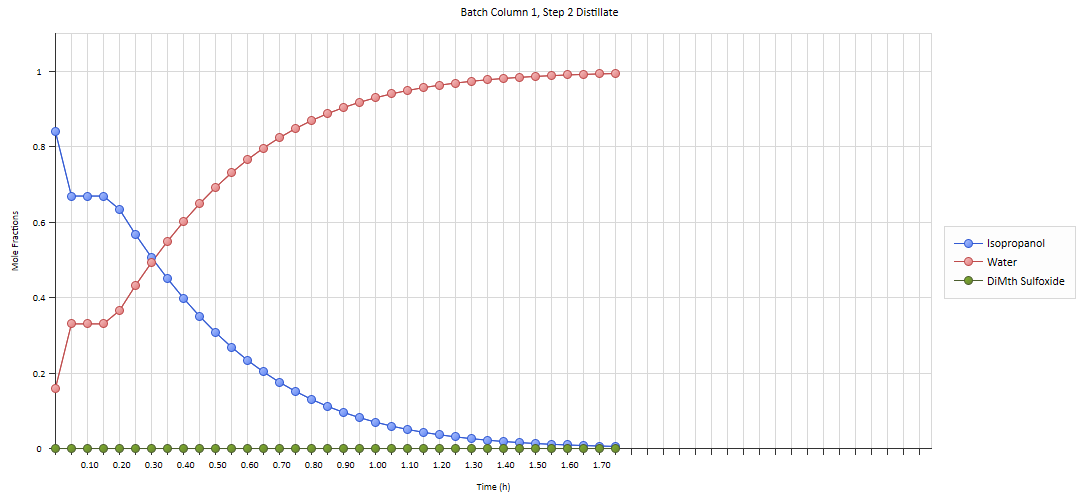
\includegraphics[width=0.8\textwidth]{figs/distgraph2.png}
\caption{Distillate composition in terms of time for step 2.}
\label{fig:Distillate composition in terms of time for step 2}
\end{figure}

\begin{figure}[H]
\centering
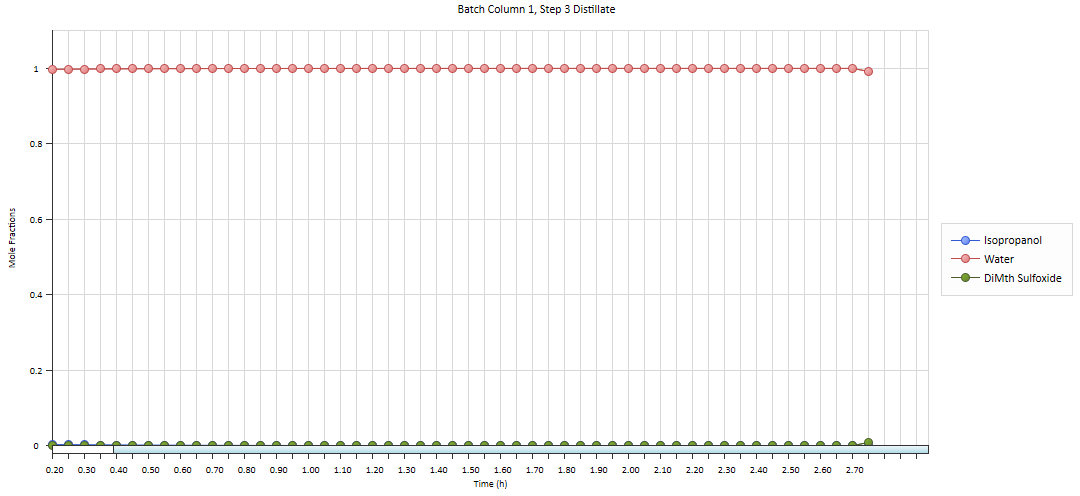
\includegraphics[width=0.8\textwidth]{figs/distgraph3.png}
\caption{Distillate composition in terms of time for step 3.}
\label{fig:Distillate composition in terms of time for step 3}
\end{figure}

\begin{figure}[H]
\centering
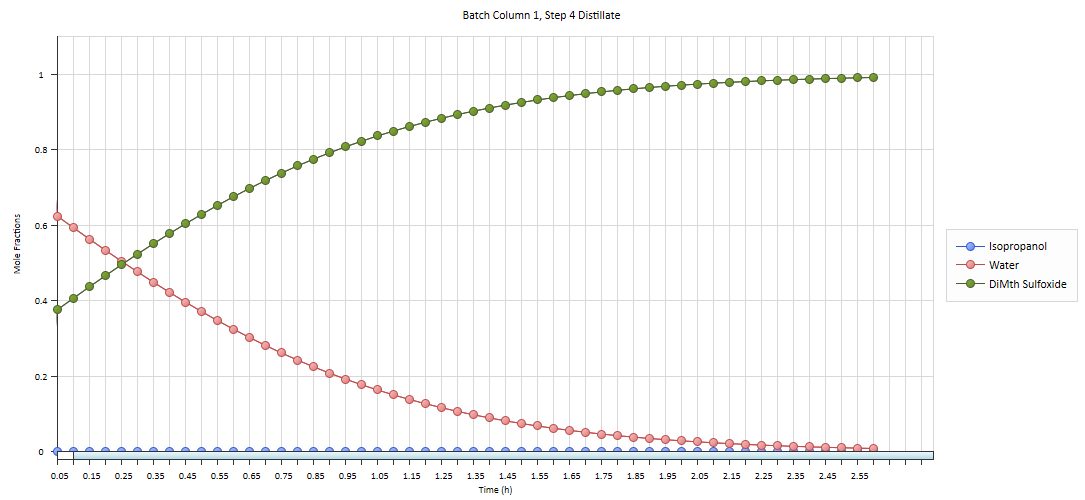
\includegraphics[width=0.8\textwidth]{figs/distgraph4.png}
\caption{Distillate composition in terms of time for step 4.}
\label{fig:Distillate composition in terms of time for step 4}
\end{figure}

After the process was finished, our results were:

\begin{itemize}
\tightlist
\item
  226.52 kg of water, 0.9994 mol fraction water
\item
  4060.02 kg of DMSO, 0.9995 mol fraction DMSO
\end{itemize}

The results are satisfying and the liquids are usable for other
applications. The total elapsed time was 16.15 hours, still under our 22
hour goal. Run-off stages will later be re-integrated into the system,
further explained in Chapter 8, in order to recover as much material as
possible. These results support the inclusion of material recovery steps
in the overall process design, as they reduce waste formation and
improve the reuse potential of both water and DMSO.

\chapter{Heat Duty}\label{heat-duty}

The distillation process requires energy, which we will want to keep at
a minimum in order not to spend resources unnecessarily. Each parameter
changes the heat duty of the operation in a different way; however, we
have set the column re-boiler's duty to be 1000 MJ/h, therefore we will
focus on how heating up the DMSO feed will affect the outcomes, which we
will calculate using a controller and a heat exchanger (via ChemCAD
simulation). We will gather data relating to the amount of energy it
takes to heat up the DMSO to a desired temperature, and how much energy
it takes to feed the column. We will add our obtained quantities to the
overall column duty and multiply by the number of hours it takes for the
process to be complete.

\begin{figure}[H]
\centering
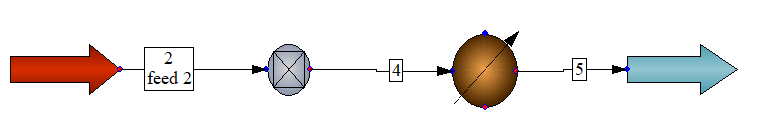
\includegraphics[width=0.5\textwidth]{figs/heatd.png}
\caption{Layout of the heat duty measurement equipment in ChemCAD.}
\label{fig:Layout of the heat duty measurement equipment in ChemCAD.}
\end{figure}

Below are the results of the conducted simulations:

\begin{figure}[H]
\centering
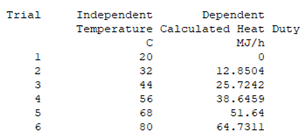
\includegraphics[width=0.5\textwidth]{figs/Picture18.png}
\caption{Effect of feed temperature on heat duty, numerical data.}
\label{fig:Effect of feed temperature on heat duty, numerical data.}
\end{figure}

\begin{longtable}[]{@{}rrr@{}}
\caption{Feed Heating Duty\\
\label{tab:Feed Heating Duty}}\tabularnewline
\toprule\noalign{}
Trial & Temperature (°C) & Calculated Heat Duty (MJ/h) \\
\midrule\noalign{}
\endfirsthead
\toprule\noalign{}
Trial & Temperature (°C) & Calculated Heat Duty (MJ/h) \\
\midrule\noalign{}
\endhead
\bottomrule\noalign{}
\endlastfoot
1 & 20 & 0 \\
2 & 32 & 12.8504 \\
3 & 44 & 25.7242 \\
4 & 56 & 38.6459 \\
5 & 68 & 51.64 \\
6 & 80 & 64.7311 \\
\end{longtable}

We can observe that raising the feed temperature from 20֯C to 62֯C will
require a heat duty of around 50 MJ/h, and it will be heated up during
the entire dIPA distillation process, which is 9.05 hours. Adding this
to our reboiler duty, which will work for 16.15 hours, we obtain 16600
MJ in total for the distillation of IPA.

\section{Energy Cost Estimation}\label{energy-cost-estimation}

The energy cost was estimated from the reboiler duty and the additional
energy required to heat the DMSO feed from 20°C to 62°C. As of 2012 in
the United States, literature reports a general electricity cost of
approximately:

\$ C\_\{\mathrm{energy}\} = 16.8~\textdollar / \mathrm{GJ} \$

This value was used as the unit energy cost for the preliminary
estimation. The energy cost was calculated by multiplying the total
energy demand by this unit cost:

\$ C = Q\_\{\mathrm{total}\} \cdot C\_\{\mathrm{energy}\} \$

For the main IPA distillation step, the reboiler operated for 9.05 h at
1000 MJ/h:

\$ Q\_\{\mathrm{reb,main}\} = 1000 \cdot 9.05 = 9050~\mathrm{MJ} =
9.05~\mathrm{GJ} \$

The DMSO feed-heating duty was approximately 50 MJ/h. Since the feed is
heated during the main distillation step:

\$ Q\_\{\mathrm{feed}\} = 50 \cdot 9.05 = 452.5~\mathrm{MJ} =
0.4525~\mathrm{GJ} \$

Therefore, the total energy required for the main IPA distillation step
was:

\$ Q\_\{\mathrm{main,total}\} = 9.05 + 0.4525 = 9.5025~\mathrm{GJ} \$

\$ C\_\{\mathrm{main}\} = 9.5025 \cdot 16.8 = 159.64~\textdollar \$

For the complete process, with a total elapsed time of 16.15 h:

\$ Q\_\{\mathrm{reb,total}\} = 1000 \cdot 16.15 = 16150~\mathrm{MJ} =
16.15~\mathrm{GJ} \$

Adding the same feed-heating energy:

\$ Q\_\{\mathrm{process,total}\} = 16.15 + 0.4525 = 16.6025~\mathrm{GJ}
\$

\$ C\_\{\mathrm{process}\} = 16.6025 \cdot 16.8 = 278.92~\textdollar \$

Therefore, using the energy cost reported by literature {[}cite{]}, the
estimated energy cost is approximately 159.64 \(\textdollar\) for the
main IPA distillation step and 278.92 \(\textdollar\) for the complete
process.

\chapter{Column Geometry}\label{column-geometry}

Our next step is to calculate the main dimensions of our column; that
is, its column diameter, tank diameter, volume, height and thickness. In
order to do this, we will need to obtain the flow rate of the vapour
phase and the density of both the vapour and liquid phases in every
stage throughout the column. This data can be obtained from the ChemCAD
software, given by the tray analysis report.

\section{F-factor and HETP value}\label{f-factor-and-hetp-value}

The F factor is a parameter that represents the momentum of our vapour
phase. From the Sulzer packing catalogue, we have picked the structured
MellapakPlusTM 252.Y packing, as has a high efficiency for atmospheric
pressure distillation {[}add citation here{]}. In the same catalogue, it
is possible to see the HETP-F factor graphs for each packing type, from
which we will pick a safe F factor that will not cause flooding or
weeping in our column. We selected 2 √Pa. {[}cite{]}

\begin{figure}[H]
\centering
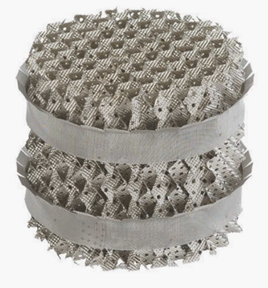
\includegraphics[width=0.3\textwidth]{figs/packpic.png}
\caption{MellapakPlus packing.}
\label{fig:MellapakPlus packing.}
\end{figure}

In the same catalogue section, we have a graph indicating what HETP
(Height Equivalent to one Theoretical Plate) value corresponds to an F
factor of 2: 0.4 m (see figure ?). The blue line refers to the
distillation pressure in mbar.

\begin{figure}[H]
\centering
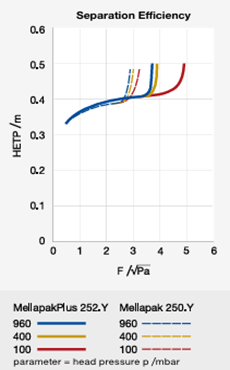
\includegraphics[width=0.5\textwidth]{figs/sulz.png}
\caption{HETP as a function of F-factor for MellapakPlus.}
\label{fig:HETP as a function of F-factor for MellapakPlus.}
\end{figure}

\section{Pressure Jump}\label{pressure-jump}

{[}add an introduction and general formula{]}

However, in the Sulzer catalogue's MellapakPlusTM 252.Y packing section,
a relationship between {[}x and y{]} is already provided:

{[}add pressure jump graph from sulzer{]}

{[}add conclusion{]}

\section{Column Height}\label{column-height}

Since the HETP value is known, the calculation of the column height can
be carried out directly. HETP stands for Height Equivalent to one
Theoretical Plate, and represents the height of packing required to
achieve the separation effect of one theoretical stage.

The column height is calculated using the following equation {[}cite
lecture{]}:

\(H = N \times HETP\)

where:

\begin{itemize}
\tightlist
\item
  \(H\) = packed column height, in m
\item
  \(N\) = number of theoretical stages
\item
  \(HETP\) = height equivalent to one theoretical plate, in m
\end{itemize}

From the previous parameter selection, the column was chosen to have 24
theoretical stages. Therefore:

\(N = 24\)

The selected HETP value for the chosen packing is:

\(HETP = 0.4 \text{m}\)

Therefore, the required packed height is:

\(H = 24 \times 0.4\)

\(H = 9.6 \text{ m}\)

The selected column height is 9.6 m, which can be rounded up to 10 m to
allow for some extra safety space.

\section{Column Diameter}\label{column-diameter}

In order to calculate the diameter of the column, the vapour phase
density in each stage must first be evaluated. This is necessary to
determine the maximum allowable vapour velocity inside the column. The
vapour velocity is calculated using the F-factor equation {[}cite{]}:

\begin{equation}{ F = v \sqrt{\rho_v} }\end{equation}

Solving for the vapour velocity:

\begin{equation}{ v = \frac{F}{\sqrt{\rho_v}} }\end{equation}

where:

\begin{itemize}
\tightlist
\item
  \texttt{F} = F-factor, in \texttt{sqrt(Pa)}
\item
  \texttt{v} = maximum vapour velocity, in \texttt{m/s}
\item
  \texttt{rho\_v} = vapour phase density, in \texttt{kg/m\^{}3}
\end{itemize}

{[}fix symbol{]}

With the vapour velocity, the cross-sectional area of the column can be
calculated by rearranging the continuity equation:

\begin{equation}{ A = \frac{\dot{V}}{v} }\end{equation}

where:

\begin{itemize}
\tightlist
\item
  \texttt{A} = cross-sectional area of the column, in \texttt{m\^{}2}
\item
  \texttt{V\_dot} = vapour volumetric flow rate, in \texttt{m\^{}3/s}
\item
  \texttt{v} = vapour velocity, in \texttt{m/s}
\end{itemize}

{[}fix symbol{]}

The column diameter is then calculated from the circular area equation:

\begin{equation}{ A = \frac{\pi D^2}{4} }\end{equation}

Solving for the diameter:

\begin{equation}{ D = \sqrt{\frac{4A}{\pi}} }\end{equation}

For each stage of the process, the highest vapour volumetric flow rate
and the lowest vapour density were considered in order to calculate the
largest required column diameter. This approach was used for safety
reasons, since the column must be able to operate under the most
demanding vapour-flow conditions.

\begin{longtable}[]{@{}
  >{\raggedright\arraybackslash}p{(\linewidth - 14\tabcolsep) * \real{0.2197}}
  >{\raggedright\arraybackslash}p{(\linewidth - 14\tabcolsep) * \real{0.1742}}
  >{\raggedright\arraybackslash}p{(\linewidth - 14\tabcolsep) * \real{0.1439}}
  >{\raggedright\arraybackslash}p{(\linewidth - 14\tabcolsep) * \real{0.1591}}
  >{\raggedright\arraybackslash}p{(\linewidth - 14\tabcolsep) * \real{0.0758}}
  >{\raggedright\arraybackslash}p{(\linewidth - 14\tabcolsep) * \real{0.0909}}
  >{\raggedright\arraybackslash}p{(\linewidth - 14\tabcolsep) * \real{0.0606}}
  >{\raggedright\arraybackslash}p{(\linewidth - 14\tabcolsep) * \real{0.0758}}@{}}
\caption{Diameter calculation results.
\label{tab:Diameter calculation results}}\tabularnewline
\toprule\noalign{}
\begin{minipage}[b]{\linewidth}\raggedright
Vapour vol.~flow rate {[}m\^{}3/s{]}
\end{minipage} & \begin{minipage}[b]{\linewidth}\raggedright
Vapour density {[}kg/m\^{}3{]}
\end{minipage} & \begin{minipage}[b]{\linewidth}\raggedright
F-factor {[}sqrt(Pa){]}
\end{minipage} & \begin{minipage}[b]{\linewidth}\raggedright
Vapour velocity {[}m/s{]}
\end{minipage} & \begin{minipage}[b]{\linewidth}\raggedright
Area {[}m\^{}2{]}
\end{minipage} & \begin{minipage}[b]{\linewidth}\raggedright
Diameter {[}m{]}
\end{minipage} & \begin{minipage}[b]{\linewidth}\raggedright
HETP {[}m{]}
\end{minipage} & \begin{minipage}[b]{\linewidth}\raggedright
Height {[}m{]}
\end{minipage} \\
\midrule\noalign{}
\endfirsthead
\toprule\noalign{}
\begin{minipage}[b]{\linewidth}\raggedright
Vapour vol.~flow rate {[}m\^{}3/s{]}
\end{minipage} & \begin{minipage}[b]{\linewidth}\raggedright
Vapour density {[}kg/m\^{}3{]}
\end{minipage} & \begin{minipage}[b]{\linewidth}\raggedright
F-factor {[}sqrt(Pa){]}
\end{minipage} & \begin{minipage}[b]{\linewidth}\raggedright
Vapour velocity {[}m/s{]}
\end{minipage} & \begin{minipage}[b]{\linewidth}\raggedright
Area {[}m\^{}2{]}
\end{minipage} & \begin{minipage}[b]{\linewidth}\raggedright
Diameter {[}m{]}
\end{minipage} & \begin{minipage}[b]{\linewidth}\raggedright
HETP {[}m{]}
\end{minipage} & \begin{minipage}[b]{\linewidth}\raggedright
Height {[}m{]}
\end{minipage} \\
\midrule\noalign{}
\endhead
\bottomrule\noalign{}
\endlastfoot
0.492 & 1.625 & 2 & 1.5689 & 0.193 & 0.496 & 0.4 & 9.6 \\
0.174 & 0.853 & 2 & 2.1655 & 0.094 & 0.346 & 0.4 & 9.6 \\
0.210 & 0.595 & 2 & 2.5928 & 0.136 & 0.416 & 0.4 & 9.6 \\
0.215 & 0.593 & 2 & 2.5972 & 0.140 & 0.422 & 0.4 & 9.6 \\
0.240 & 2.100 & 2 & 1.3801 & 0.083 & 0.325 & 0.4 & 9.6 \\
\end{longtable}

As shown in Table ?, the highest calculated diameter value is 0.495689
m. This value can be rounded up to 0.5 m. To provide an additional
safety margin, a safety factor of 20\% is applied {[}cite{]}:

\begin{equation}{ D\_{\text{selected}} = 0.50 \times 1.20 = 0.60 \text{ m} }\end{equation}

Therefore, the final selected column diameter is 60 m.

\section{Column Thickness}\label{column-thickness}

The wall thickness of the distillation column was calculated by treating
the column as a cylindrical pressure vessel under internal pressure. For
safety purposes, the design pressure was selected as 6 bar, which is
higher than the expected operating pressure of the column. The column is
assumed to be made of carbon steel, with an allowable stress of
\(S = 120 \times 10^6 \text{ Pa}\) and a weld joint efficiency of
\(E = 0.85\). {[}cite{]}

The minimum required wall thickness was calculated using the cylindrical
vessel equation {[}cite{]}:

\(t = \frac{P R}{S E - 0.6P}\)

where:

\begin{itemize}
\tightlist
\item
  \(t\) = minimum required wall thickness, in m
\item
  \(P\) = design pressure, in Pa
\item
  \(R\) = internal radius of the column, in m
\item
  \(S\) = allowable stress of the construction material, in Pa
\item
  \(E\) = weld joint efficiency
\end{itemize}

For this calculation, the following values were used:

\begin{longtable}[]{@{}llll@{}}
\caption{Parameters relevant to wall thickness.
\label{tab:wall thickness}}\tabularnewline
\toprule\noalign{}
Parameter & Symbol & Value & Unit \\
\midrule\noalign{}
\endfirsthead
\toprule\noalign{}
Parameter & Symbol & Value & Unit \\
\midrule\noalign{}
\endhead
\bottomrule\noalign{}
\endlastfoot
Design pressure & \(P\) & 600000 & Pa \\
Column diameter & \(D\) & 0.60 & m \\
Column radius & \(R\) & 0.30 & m \\
Allowable stress of carbon steel & \(S\) & \(120 \times 10^6\) & Pa \\
Weld joint efficiency & \(E\) & 0.85 & - \\
\end{longtable}

Substituting the values:

\(t = \frac{600000 \times 0.30}{(120 \times 10^6)(0.85) - 0.6(600000)}\)

\(t = 0.00177 \text{ m}\)

\(t = 1.77 \text{ mm}\)

The calculated theoretical wall thickness is therefore 1.77 mm. However,
this value only represents the minimum thickness required to withstand
the selected internal design pressure. A corrosion allowance must also
be included, especially because carbon steel is used as the construction
material. Assuming a corrosion allowance of 3.2 mmc{[}cite book{]}:

\(t_{\text{final}} = t + C_A\)

\(t_{\text{final}} = 1.77 + 3.2\)

\(t_{\text{final}} = 4.97 \text{ mm}\)

Therefore, the selected practical wall thickness is rounded up to:

\(t_{\text{selected}} = 5 \text{ mm}\)

The final selected wall thickness of the column for the 6 bar internal
pressure case is therefore 5 mm.

The column is also later planned to withstand an internal pressure of
0.1 bar. Since the outside of the column is assumed to be at atmospheric
pressure, this condition creates an external pressure difference of
approximately \(P_{\text{external}} = 1.013 - 0.1 = 0.913 \text{ bar}\).
This case must be checked separately, because vacuum operation is
controlled by external pressure collapse rather than internal pressure
stress.

A preliminary external pressure check shows that a 5 mm wall thickness
can withstand the vacuum condition if the full 5 mm thickness is
available structurally:

{[}add external pressure check calculations{]}

However, if the 5 mm thickness includes a 3.2 mm corrosion allowance,
the effective structural thickness would be only 1.8 mm, which is not
sufficient for the 0.1 bar internal pressure case. Therefore, if vacuum
operation at 0.1 bar must be guaranteed while keeping the 3.2 mm
corrosion allowance, a larger nominal wall thickness, such as 7 mm, is
recommended.

\section{Tank Geometry}\label{tank-geometry}

The tank geometry was determined based on the maximum liquid volume
obtained from the simulation results. From the tank volume values, the
maximum required volume was approximately:

\(V_{\text{max}} = 6 \text{ m}^3\)

In order to provide an additional safety margin for bubbling and avoid
operating the tank exactly at its maximum capacity, a larger geometrical
volume was selected. The tank was designed as a vertical cylindrical
vessel with a height of 2.5 m and a diameter of 2.0 m.

The volume of a cylindrical tank is calculated as:

\(V = \frac{\pi D^2}{4}H\)

where:

\begin{itemize}
\tightlist
\item
  \(V\) = tank volume, in m³
\item
  \(D\) = tank diameter, in m
\item
  \(H\) = tank height, in m
\end{itemize}

Substituting the selected dimensions:

\(V = \frac{\pi (2.0)^2}{4}(2.5)\)

\(V = 7.85 \text{ m}^3\)

Therefore, the selected tank dimensions provide a total geometrical
volume of approximately 7.85 m\^{}3.

Since this value is greater than the maximum required process volume of
6 m³, the selected tank geometry provides sufficient additional capacity
for safe operation. The final selected tank dimensions are therefore:

\begin{longtable}[]{@{}lrrr@{}}
\caption{Final Dimensions of the column tank.
\label{tab:Final Dimensions of the column tank}}\tabularnewline
\toprule\noalign{}
Parameter & Symbol & Value & Unit \\
\midrule\noalign{}
\endfirsthead
\toprule\noalign{}
Parameter & Symbol & Value & Unit \\
\midrule\noalign{}
\endhead
\bottomrule\noalign{}
\endlastfoot
Maximum required volume & \(V_{\text{max}}\) & 6.00 & m³ \\
Selected tank diameter & \(D\) & 2.00 & m \\
Selected tank height & \(H\) & 2.50 & m \\
Selected tank volume & \(V_{\text{tank}}\) & 7.85 & m³ \\
\end{longtable}

\chapter{Heat Exchangers}\label{heat-exchangers-1}

\section{Column Condenser Design}\label{column-condenser-design}

The condenser was designed as a one-pass shell-and-tube heat exchanger
used to condense the IPA-rich vapour leaving the top of the distillation
column.

{[}add paragraph explaining why one pass heat exchanger is good{]}

The total heat-transfer area listed in the calculation corresponds to
the total available outside tube surface area. The IPA properties used
for the condensation-side calculation were obtained from ChemCAD's
reports, while the cooling-water properties were taken at the average
cooling-water temperature in a different ChemCAD simulation arrangement.

{[}add graph or reports from chemcad{]}

{[}add simulation arrangement picture{]}

The main design equation used for the condenser was:

\(Q = K F A \Delta T_m\)

Rearranging for the required heat-transfer area:

\(A = \frac{Q}{F}{K \Delta T_m}\)

where \(Q\) is the condenser heat duty, \(K\) is the overall
heat-transfer coefficient, \(A\) is the total heat-transfer area, \(F\)
is the correction factor and \(\Delta T_m\) is the mean temperature
difference. Since the temperature difference between the condensing
vapour and cooling water changes along the exchanger, the logarithmic
mean temperature difference was used:

\(\Delta T_{log} = \frac{\Delta T_1 - \Delta T_2}{\ln \left(\frac{\Delta T_1}{\Delta T_2}\right)}\)

The IPA vapour was assumed to condense at constant temperature since we
are dealing with a phase change, while the cooling water was heated from
25°C (room temperature) to 50°C. Therefore:

\(\Delta T_1 = T_{IPA} - T_{w,in}\)

\(\Delta T_1 = 353.15 - 298.15 = 55 \text{ K}\)

\(\Delta T_2 = T_{IPA} - T_{w,out}\)

\(\Delta T_2 = 353.15 - 323.15 = 30 \text{ K}\)

Thus:

\(\Delta T_{log} = \frac{55 - 30}{\ln \left(\frac{55}{30}\right)}\)

\(\Delta T_{log} = 41.24 \text{ K}\)

The correction factor was calculated as:

\(F_T = 1\)

{[}add graph from book{]}

Therefore:

\(\Delta T_m = F_T \Delta T_{log}\)

\(\Delta T_m = 41.24 \text{ K}\)

The highest condenser heat duty obtained from the simulation was:

\(Q = 957.7 \text{ MJ/h}\)

{[}add picture of graph from chemcad{]}

Converting to watts:

\(Q = \frac{957.7 \times 10^6}{3600}\)

\(Q = 266027.78 \text{ W}\)

Using the initially assumed overall heat-transfer coefficient for phase
change {[}cite{]}:

\(K = 850 \text{ W/m}^2\text{K}\)

the first estimated heat-transfer area was:

\(A = \frac{266027.78}{850 \times 41.24}\)

\(A = 7.59 \text{ m}^2\)

This value was used only as an initial estimate. A corrected design was
then obtained by calculating the individual heat-transfer coefficients,
the wall resistance, and the fouling resistance.

The clean overall heat-transfer coefficient was calculated from the
thermal resistance relationship {[}cite lecture{]}:

\(\frac{1}{K_{clean}} = \frac{1}{\alpha_{w,out}} + \frac{x_{tube}}{\lambda_{wall}} + \frac{1}{\alpha_{cond}}\)

where \(\alpha_{w,out}\) is the cooling-water heat-transfer coefficient
converted to the outside tube area, \(x_{tube}\) is the tube wall
thickness, \(\lambda_{wall}\) is the thermal conductivity of the
carbon-steel wall, and \(\alpha_{cond}\) is the condensation-side
heat-transfer coefficient. The wall thermal conductivity was taken as
{[}cite{]}:

\(\lambda_{wall} = 45 \text{ W/mK}\)

The water-side Reynolds number was calculated using {[}cite lecture{]}:

\(Re = \frac{\rho v D_i}{\mu}\)

The Prandtl number was calculated using {[}cite lecture{]}:

\(Pr = \frac{\mu c_p}{\lambda}\)

The Nusselt number used in the worksheet was {[}cite lecture{]}:

\(Nu = 0.3 Re^{0.5} Pr^{1/3}\)

The water-side heat-transfer coefficient was then calculated from
{[}cite lecture{]}:

\(\alpha_{w,in} = \frac{Nu \lambda_w}{D_i}\)

Since the total heat-transfer area was based on the outside tube
surface, the water-side coefficient was converted to the outside area
basis:

\(\alpha_{w,out} = \alpha_{w,in} \frac{D_i}{D_o}\)

The calculated condenser coefficients were:

\begin{longtable}[]{@{}
  >{\raggedright\arraybackslash}p{(\linewidth - 6\tabcolsep) * \real{0.5692}}
  >{\raggedleft\arraybackslash}p{(\linewidth - 6\tabcolsep) * \real{0.2462}}
  >{\raggedleft\arraybackslash}p{(\linewidth - 6\tabcolsep) * \real{0.1077}}
  >{\raggedleft\arraybackslash}p{(\linewidth - 6\tabcolsep) * \real{0.0769}}@{}}
\caption{Condenser heat transfer coefficients.
\label{tab:Condenser heat transfer coefficients.}}\tabularnewline
\toprule\noalign{}
\begin{minipage}[b]{\linewidth}\raggedright
Parameter
\end{minipage} & \begin{minipage}[b]{\linewidth}\raggedleft
Symbol
\end{minipage} & \begin{minipage}[b]{\linewidth}\raggedleft
Value
\end{minipage} & \begin{minipage}[b]{\linewidth}\raggedleft
Unit
\end{minipage} \\
\midrule\noalign{}
\endfirsthead
\toprule\noalign{}
\begin{minipage}[b]{\linewidth}\raggedright
Parameter
\end{minipage} & \begin{minipage}[b]{\linewidth}\raggedleft
Symbol
\end{minipage} & \begin{minipage}[b]{\linewidth}\raggedleft
Value
\end{minipage} & \begin{minipage}[b]{\linewidth}\raggedleft
Unit
\end{minipage} \\
\midrule\noalign{}
\endhead
\bottomrule\noalign{}
\endlastfoot
Condensation-side coefficient & \(\alpha_{cond}\) & 1995.01 & W/m²K \\
Water-side coefficient, inside basis & \(\alpha_{w,in}\) & 1514.09 &
W/m²K \\
Water-side coefficient, outside basis & \(\alpha_{w,out}\) & 1211.27 &
W/m²K \\
Clean overall coefficient & \(K_{clean}\) & 729.25 & W/m²K \\
Fouling resistance & \(R_f\) & 0.0005 & m²K/W \\
Dirty overall coefficient & \(K_{dirty}\) & 534.40 & W/m²K \\
\end{longtable}

Fouling resistance was obtained from literature {[}cite book{]}.

The dirty overall heat-transfer coefficient was calculated by adding the
fouling resistance:

\(\frac{1}{K_{dirty}} = \frac{1}{K_{clean}} + R_f\)

\(K_{dirty} = 534.40 \text{ W/m}^2\text{K}\)

Using the dirty overall heat-transfer coefficient, the final required
heat-transfer area was:

\(A_{calc} = \frac{Q}{K_{dirty} \Delta T_{log}}\)

\(A_{calc} = \frac{266027.78}{534.40 \times 41.24}\)

\(A_{calc} = 12.07 \text{ m}^2\)

Therefore, the required total condenser heat-transfer area is:

\(A_{cond} = 12.07 \text{ m}^2\)

The selected condenser geometry was:

\begin{longtable}[]{@{}lrrr@{}}
\caption{Selected and calculated condenser geometry.
\label{tab:Selected and calculated condenser geometry}}\tabularnewline
\toprule\noalign{}
Parameter & Symbol & Value & Unit \\
\midrule\noalign{}
\endfirsthead
\toprule\noalign{}
Parameter & Symbol & Value & Unit \\
\midrule\noalign{}
\endhead
\bottomrule\noalign{}
\endlastfoot
Number of tubes & \(N\) & 48 & - \\
Tube outside diameter & \(D_o\) & 0.020 & m \\
Tube inside diameter & \(D_i\) & 0.016 & m \\
Tube wall thickness & \(x_{tube}\) & 0.002 & m \\
Tube pitch & \(p_t\) & 0.025 & m \\
Tube length & \(L\) & 4.002 & m \\
Bundle diameter & \(D_{bundle}\) & 0.232 & m \\
Shell clearance & - & 0.011 & m \\
Shell inside diameter & \(D_{shell,in}\) & 0.243 & m \\
Shell wall thickness & \(x_{shell}\) & 0.00423 & m \\
Shell length & \(L_{shell}\) & 4.028 & m \\
Baffle spacing & - & 0.0486 & m \\
\end{longtable}

The tube outside diameter, tube thickness, tube pitch and shell
clearance values were amongst those recommended by literature {[}cite
book{]}. Similarly, the formulas for the bundle diameter, shell
thickness, shell diameter and and shell length were given:

{[}give four formulas{]}

The number of tubes was arbitrarily selected to comply with length
recommendations and the chosen arrangement. Inversely, tube length was
calculated with the following formula {[}cite lecture{]}:

\begin{equation}{L = \frac{A}{N \pi D_o}}\end{equation}

The tube arrangement {[}add explanation indicating why 2x2 is
suitable{]}.

{[}add picture of chosen arrangement{]}

The available outside tube surface area was checked using:

\(A = N \pi D_o L\)

\(A = 48 \pi (0.020)(4.002)\)

\(A = 12.07 \text{ m}^2\)

Therefore, the selected condenser geometry provides the required total
heat-transfer area.

The cooling-water mass flow rate was calculated from the sensible heat
balance {[}cite lecture{]}:

\(Q = \dot{m}_w c_{p,w} \Delta T_w\)

\(\dot{m}_w = \frac{Q}{c_{p,w} \Delta T_w}\)

The calculated cooling-water mass flow rate was:

\(\dot{m}_w = 2.55 \text{ kg/s}\)

The main hydraulic results for the cooling water were:

\begin{longtable}[]{@{}lrrr@{}}
\caption{Cooling water properties.
\label{tab:Cooling water properties}}\tabularnewline
\toprule\noalign{}
Parameter & Symbol & Value & Unit \\
\midrule\noalign{}
\endfirsthead
\toprule\noalign{}
Parameter & Symbol & Value & Unit \\
\midrule\noalign{}
\endhead
\bottomrule\noalign{}
\endlastfoot
Water mass flow rate & \(\dot{m}_w\) & 2.55 & kg/s \\
Tube-side flow area & \(A_{tube}\) & 0.00965 & m² \\
Water velocity & \(v_w\) & 0.266 & m/s \\
Reynolds number & \(Re_w\) & 5876.23 & - \\
Prandtl number & \(Pr_w\) & 4.81 & - \\
Nusselt number & \(Nu_w\) & 38.82 & - \\
\end{longtable}

The calculated wall and film temperatures were:

\begin{longtable}[]{@{}
  >{\raggedright\arraybackslash}p{(\linewidth - 6\tabcolsep) * \real{0.4355}}
  >{\raggedleft\arraybackslash}p{(\linewidth - 6\tabcolsep) * \real{0.4194}}
  >{\raggedleft\arraybackslash}p{(\linewidth - 6\tabcolsep) * \real{0.0806}}
  >{\raggedleft\arraybackslash}p{(\linewidth - 6\tabcolsep) * \real{0.0645}}@{}}
\caption{Condenser wall and film temperatures.
\label{tab:Condenser wall and film temperatures}}\tabularnewline
\toprule\noalign{}
\begin{minipage}[b]{\linewidth}\raggedright
Parameter
\end{minipage} & \begin{minipage}[b]{\linewidth}\raggedleft
Symbol
\end{minipage} & \begin{minipage}[b]{\linewidth}\raggedleft
Value
\end{minipage} & \begin{minipage}[b]{\linewidth}\raggedleft
Unit
\end{minipage} \\
\midrule\noalign{}
\endfirsthead
\toprule\noalign{}
\begin{minipage}[b]{\linewidth}\raggedright
Parameter
\end{minipage} & \begin{minipage}[b]{\linewidth}\raggedleft
Symbol
\end{minipage} & \begin{minipage}[b]{\linewidth}\raggedleft
Value
\end{minipage} & \begin{minipage}[b]{\linewidth}\raggedleft
Unit
\end{minipage} \\
\midrule\noalign{}
\endhead
\bottomrule\noalign{}
\endlastfoot
Real wall temperature & \(\overline{T}_{wall,real}\) & 68.62 & °C \\
Calculated wall temperature & \(\overline{T}_{wall,calc}\) & 70.00 &
°C \\
Film temperature & \(\overline{T}_{film}\) & 75.00 & °C \\
\end{longtable}

From the formulas {[}cite lectures{]}:

{[}add 2 formulas{]}

The value of the film temperature was chosen by iteration, performed
until the calculated wall temperature was close to the real wall
temperature. A normal temperature difference interval between the film
and wall temperatures is of around 5 to 10 degrees.

The small difference between the real and calculated wall temperatures
shows that the assumed film temperature is acceptable for the
preliminary condenser design. All other calculated parameters are
realistic for the scale of our process and adequate for manufacturing
{[}cite{]}.

\section{Column Reboiler Design}\label{column-reboiler-design}

The reboiler was designed as a kettle reboiler. Although it is not a
traditional shell-and-tube heat exchanger in the same way as the
condenser, it still uses a tube bundle to transfer heat from condensing
steam to the process liquid. The reboiler was designed as a two-pass
heat exchanger arrangement, with the listed heat-transfer area
representing the total heat-transfer area.

{[}add paragraph explaining why kettle reboiler is good{]} {[}cite{]}

The DMSO-rich liquid properties were obtained from ChemCAD using the
relevant column-bottom composition, while the steam-side properties were
obtained from a saturated steam table by interpolation {[}cite steam
table{]}.

In this case, it was not necessary to calculate the logarithmic
temperature difference, since we chose the steam temperature.
Furthermore, the heat duty is known.

{[}add picture of chemcad graph for reboiler{]}

{[}add picture of steam stable{]}

{[}add interpolation formula{]}

The design equation used for the reboiler was:

\(Q = K A \Delta T\) F

Rearranging for heat-transfer area:

\(A = \frac{Q}{K \Delta T}\)

The DMSO-rich liquid temperature was taken as:

\(T_{DMSO} = 190^\circ C\)

The heating steam temperature was taken as:

\(T_{steam} = 220^\circ C\)

For an adequate temperature difference of:

\(\Delta T = T_{steam} - T_{DMSO}\)

\(\Delta T = 220 - 190\)

\(\Delta T = 30 \text{ K}\)

This will allow for proper heat transfer without overheating the DMSO,
which properties we will take as reference since it possesses the
highest heat transfer resistance ({[}add heat transfer coefficients of
water, IPA and DMSO{]}) {[}add citation{]}. For stages where DMSO does
not make up most of the bottom liquid, the pressure of steam (and
therefore the temperature) is to be decreased with a control system. At
higher temperatures, a peak and then a rapid decrease in the value of
the heat transfer coefficient can be observed {[}cite hegelys book from
picture{]}.

{[}add picture of graph from book{]}

The reboiler heat duty was:

\(Q = 1000 \text{ MJ/h}\)

Converting to watts:

\(Q = \frac{1000 \times 10^6}{3600}\)

\(Q = 277777.78 \text{ W}\)

Using the initially assumed overall heat-transfer coefficient for phase
change {[}cite book{]}:

\(K = 850 \text{ W/m}^2\text{K}\)

the preliminary heat-transfer area was:

\(A = \frac{277777.78}{850 \times 30}\)

\(A = 10.89 \text{ m}^2\)

This initial estimate was corrected by calculating the individual
boiling-side and steam-condensation-side heat-transfer coefficients.

The boiling-side heat-transfer coefficient for the process was
calculated using the pool-boiling correlation {[}cite book{]}:

{[}add formula{]}

\(\alpha_{shell} = 2261.06 \text{ W/m}^2\text{K}\)

The steam-side condensation coefficient was calculated using the
filmwise-condensation method. The inside coefficient was first
calculated and then converted to the outside tube surface basis {[}cite
book{]}:

\(\alpha_{st,out} = \alpha_{st,in} \frac{D_i}{D_o}\)

The calculated reboiler heat-transfer coefficients were:

\begin{longtable}[]{@{}
  >{\raggedright\arraybackslash}p{(\linewidth - 6\tabcolsep) * \real{0.6000}}
  >{\raggedleft\arraybackslash}p{(\linewidth - 6\tabcolsep) * \real{0.2267}}
  >{\raggedleft\arraybackslash}p{(\linewidth - 6\tabcolsep) * \real{0.1067}}
  >{\raggedleft\arraybackslash}p{(\linewidth - 6\tabcolsep) * \real{0.0667}}@{}}
\caption{Reboiler heat transfer coefficients.
\label{tab:Reboiler heat transfer coefficients}}\tabularnewline
\toprule\noalign{}
\begin{minipage}[b]{\linewidth}\raggedright
Parameter
\end{minipage} & \begin{minipage}[b]{\linewidth}\raggedleft
Symbol
\end{minipage} & \begin{minipage}[b]{\linewidth}\raggedleft
Value
\end{minipage} & \begin{minipage}[b]{\linewidth}\raggedleft
Unit
\end{minipage} \\
\midrule\noalign{}
\endfirsthead
\toprule\noalign{}
\begin{minipage}[b]{\linewidth}\raggedright
Parameter
\end{minipage} & \begin{minipage}[b]{\linewidth}\raggedleft
Symbol
\end{minipage} & \begin{minipage}[b]{\linewidth}\raggedleft
Value
\end{minipage} & \begin{minipage}[b]{\linewidth}\raggedleft
Unit
\end{minipage} \\
\midrule\noalign{}
\endhead
\bottomrule\noalign{}
\endlastfoot
Boiling-side coefficient & \(\alpha_{shell}\) & 2261.06 & W/m²K \\
Steam condensation coefficient, inside basis & \(\alpha_{st,in}\) &
12152.33 & W/m²K \\
Steam condensation coefficient, outside basis & \(\alpha_{st,out}\) &
10194.74 & W/m²K \\
Clean overall coefficient & \(K_{clean}\) & 1708.92 & W/m²K \\
Fouling resistance & \(R_f\) & 0.00026 & m²K/W \\
Dirty overall coefficient & \(K_{dirty}\) & 1183.20 & W/m²K \\
\end{longtable}

The clean overall heat-transfer coefficient was calculated as:

\(\frac{1}{K_{clean}} = \frac{1}{\alpha_{st,out}} + \frac{x_{tube}}{\lambda_{wall}} + \frac{1}{\alpha_{shell}}\)

The dirty overall heat-transfer coefficient was calculated by including
the fouling resistance {[}cite book{]}:

\(\frac{1}{K_{dirty}} = \frac{1}{K_{clean}} + R_f\)

\(K_{dirty} = 1183.20 \text{ W/m}^2\text{K}\)

The correction factor was calculated for a two-pass heat exchanger:

{[}add correction factor formula{]}

{[}add picture of graph from book{]}

Using the dirty overall coefficient, the corrected reboiler
heat-transfer area was:

\(A_{calc} = \frac{Q}{F}{K_{dirty} \Delta T}\)

\(A_{calc} = \frac{277777.78}{1}{1183.20 \times 30}\)

\(A_{calc} = 7.83 \text{ m}^2\)

Therefore, the required total reboiler heat-transfer area is:

\(A_{reb} = 7.83 \text{ m}^2\)

The selected reboiler geometry was:

\begin{longtable}[]{@{}lrrr@{}}
\caption{Selected and calculated reboiler geometry.
\label{tab:Selected and calculated reboiler geometry}}\tabularnewline
\toprule\noalign{}
Parameter & Symbol & Value & Unit \\
\midrule\noalign{}
\endfirsthead
\toprule\noalign{}
Parameter & Symbol & Value & Unit \\
\midrule\noalign{}
\endhead
\bottomrule\noalign{}
\endlastfoot
Number of tubes & \(N\) & 28 & - \\
Tube outside diameter & \(D_o\) & 0.0250 & m \\
Tube inside diameter & \(D_i\) & 0.0210 & m \\
Tube wall thickness & \(x_{tube}\) & 0.00202 & m \\
Tube pitch & \(p_t\) & 0.0313 & m \\
Tube length & \(L\) & 1.777 & m \\
Bundle diameter & \(D_{bundle}\) & 0.227 & m \\
Shell clearance & - & 0.011 & m \\
Shell inside diameter & \(D_{shell,in}\) & 0.477 & m \\
Shell wall thickness & \(x_{shell}\) & 0.00493 & m \\
\end{longtable}

The tube length was calculated from the total required heat-transfer
area:

\(L = \frac{A}{2N \pi D_o}\)

The factor of 2 is included because the reboiler was designed with a
two-pass tube arrangement {[}cite lecture{]}.

Substituting the values:

\(L = \frac{7.83}{2(28)\pi(0.0250)}\)

\(L = 1.78 \text{ m}\)

Therefore, the selected tube length is 1.78 m.

The steam mass flow rate was calculated from the latent heat balance:

\(Q = \dot{m}_{st} r_{st}\)

\(\dot{m}_{st} = \frac{Q}{r_{st}}\)

The latent heat of the heating steam was obtained from the steam table
by interpolation:

\(r_{st} = 1887700 \text{ J/kg}\)

Therefore:

\(\dot{m}_{st} = \frac{277777.78}{1887700}\)

\(\dot{m}_{st} = 0.147 \text{ kg/s}\)

The main steam-side hydraulic values were:

\begin{longtable}[]{@{}lrrr@{}}
\caption{Steam parameters. \label{tab:Steam parameters}}\tabularnewline
\toprule\noalign{}
Parameter & Symbol & Value & Unit \\
\midrule\noalign{}
\endfirsthead
\toprule\noalign{}
Parameter & Symbol & Value & Unit \\
\midrule\noalign{}
\endhead
\bottomrule\noalign{}
\endlastfoot
Steam mass flow rate & \(\dot{m}_{st}\) & 0.147 & kg/s \\
Tube-side flow area & \(A_{tube}\) & 0.00485 & m² \\
Steam velocity & \(v_{st}\) & 2.95 & m/s \\
\end{longtable}

The calculated wall and film temperatures were obtained from the formula
{[}cite lecture{]}:

{[}add formula{]}

The results could be summarized below:

\begin{longtable}[]{@{}
  >{\raggedright\arraybackslash}p{(\linewidth - 6\tabcolsep) * \real{0.4286}}
  >{\raggedleft\arraybackslash}p{(\linewidth - 6\tabcolsep) * \real{0.4127}}
  >{\raggedleft\arraybackslash}p{(\linewidth - 6\tabcolsep) * \real{0.0952}}
  >{\raggedleft\arraybackslash}p{(\linewidth - 6\tabcolsep) * \real{0.0635}}@{}}
\caption{Reboiler wall and film temperatures.
\label{tab:Reboiler wall and film temperatures}}\tabularnewline
\toprule\noalign{}
\begin{minipage}[b]{\linewidth}\raggedright
Parameter
\end{minipage} & \begin{minipage}[b]{\linewidth}\raggedleft
Symbol
\end{minipage} & \begin{minipage}[b]{\linewidth}\raggedleft
Value
\end{minipage} & \begin{minipage}[b]{\linewidth}\raggedleft
Unit
\end{minipage} \\
\midrule\noalign{}
\endfirsthead
\toprule\noalign{}
\begin{minipage}[b]{\linewidth}\raggedright
Parameter
\end{minipage} & \begin{minipage}[b]{\linewidth}\raggedleft
Symbol
\end{minipage} & \begin{minipage}[b]{\linewidth}\raggedleft
Value
\end{minipage} & \begin{minipage}[b]{\linewidth}\raggedleft
Unit
\end{minipage} \\
\midrule\noalign{}
\endhead
\bottomrule\noalign{}
\endlastfoot
Real wall temperature & \(\overline{T}_{wall,real}\) & 204.30 & °C \\
Calculated wall temperature & \(\overline{T}_{wall,calc}\) & 205.00 &
°C \\
Film temperature & \(\overline{T}_{film}\) & 212.50 & °C \\
\end{longtable}

The small difference between the real and calculated wall temperatures
confirms that the assumed film temperature is acceptable for the
preliminary kettle reboiler calculation.

All calculated parameters are realistic for the scale of our process and
adequate for the manufacturing of parts for this reboiler {[}cite{]}.

\section{Selection of Heat Exchanger Construction
Types}\label{selection-of-heat-exchanger-construction-types}

The condenser was selected as a conventional one-pass shell-and-tube
heat exchanger. Since the exchanger is relatively small and the
temperature difference is moderate, a fixed-tube-sheet construction is
suitable. For the front-end stationary head, a removable channel and
cover is selected so that the tube side can be accessed for inspection
and cleaning. The selected front-end type is therefore TEMA type A
{[}cite book{]}. The shell is selected as a one-pass shell,
corresponding to TEMA shell type E. The rear-end head is selected as a
fixed-tube-sheet rear channel with removable cover, corresponding to
TEMA rear-end type L. Therefore, the selected condenser construction is:

\(AEL\)

where:

\begin{itemize}
\tightlist
\item
  \(A\) = front-end stationary head with removable channel and cover
\item
  \(E\) = one-pass shell
\item
  \(L\) = fixed-tube-sheet rear end with removable cover
\end{itemize}

{[}add picture of table{]}

This construction is appropriate for a normal one-pass condenser because
it is mechanically simple, allows tube-side access, and provides the
required heat-transfer area.

The reboiler was selected as a kettle-type reboiler rather than a
conventional shell-and-tube heat exchanger. For this reason, the shell
type must correspond to a kettle arrangement. The selected shell type is
therefore TEMA type K. Since the reboiler uses a two-pass tube
arrangement and must allow thermal expansion of the tube bundle, a
U-tube rear-end construction is suitable. The selected rear-end type is
TEMA type U. For the front-end stationary head, a bonnet-type head is
selected because the tube-side fluid is condensing steam, which is
relatively clean compared with process liquids. The selected front-end
type is therefore TEMA type B. Therefore, the selected reboiler
construction is:

\(BKU\)

where:

\begin{itemize}
\tightlist
\item
  \(B\) = bonnet-type front-end stationary head
\item
  \(K\) = kettle-type shell
\item
  \(U\) = U-tube rear-end construction
\end{itemize}

This construction is appropriate for the kettle reboiler because the
kettle shell provides space for boiling and vapour-liquid disengagement,
while the U-tube arrangement allows thermal expansion and provides the
required two-pass tube-side flow path.

{[}add picture of kettle reboiler{]}

\chapter{Material Recovery}\label{material-recovery}

After the main batch extractive distillation step, two secondary run-off
streams are produced: an IPA/water run-off and a water/DMSO run-off.
These streams do not meet the purity requirements to be considered final
products, but they still contain recoverable amounts of IPA, water, and
DMSO. Therefore, instead of treating them as waste, their re-integration
into later batches was studied in order to reduce material losses and
improve the overall efficiency of the process.

Two recycling strategies were compared using ChemCAD simulations. In
both cases, the results of one batch were used as input for the next
batch. Batch 1 corresponds to the original reference batch, while
Batches 2--6 represent five consecutive recycle batches. For each batch,
the total moles, mass, purity of the run-off streams, IPA distillate
purity, distillate mass, elapsed time, and DMSO bottom-product purity
were recorded.

In the first method, only the IPA/water run-off is added to the pot
charge of the next batch, while the recovered DMSO bottom product from
the previous distillation is used as the solvent feed for the next
batch. Since the amount of recovered DMSO is lower than the amount
required for a complete new batch, the missing amount would be replaced
in practice by externally supplied, theoretically pure DMSO. However, in
the simulation, the additional pure DMSO was not included in the purity
calculation. Instead, the purity of the recovered bottom DMSO was used
as the next solvent-feed purity, representing the worst-case scenario.
The water/DMSO run-off is not directly recycled in this method and is
instead kept for later recovery distillation.

In the second method, both the IPA/water run-off and the water/DMSO
run-off are added directly to the pot charge of the next batch. This
method has the advantage of immediately reusing all run-off material,
but it also introduces more water and DMSO into the next batch, which
can influence the charge composition, separation time, and simulation
convergence.

Abbreviations:

\begin{itemize}
\tightlist
\item
  \texttt{B} = batch
\item
  \texttt{RO} = run-off
\item
  \texttt{x} = mole fraction
\item
  \texttt{m} = mass
\item
  \texttt{n} = amount of substance
\item
  \texttt{Chg.} = charge
\item
  \texttt{Dist.} = distillate
\item
  \texttt{t} = time
\end{itemize}

\section{Method 1, Water/IPA Run-off
Re-integration}\label{method-1-wateripa-run-off-re-integration}

In the first recycling method, the IPA/water run-off from each batch was
added to the pot charge of the following batch. The DMSO bottom product
from the previous batch was reused as the next batch's solvent feed. The
water/DMSO run-off was not added directly to the following batch, but
was instead collected for later recovery. This approach aims to recover
IPA-containing material without continuously increasing the amount of
DMSO in the pot charge.

The initial charge values used for this recycle sequence were 41.18112
kmol IPA and 21.21452 kmol water. During the ChemCAD simulations, some
operating adjustments were required to maintain convergence and product
purity. For Batch 2, the reflux ratio in step 3 was changed from 4 to 5.
For Batch 5, the reflux ratio in step 3 was further changed from 5 to 6.
These changes were necessary to keep the distillation within the
required purity range as the recycled material influenced the batch
composition.

\subsection{IPA/Water Run-off and IPA Distillate
Results}\label{ipawater-run-off-and-ipa-distillate-results}

\begin{longtable}[]{@{}
  >{\raggedleft\arraybackslash}p{(\linewidth - 22\tabcolsep) * \real{0.0957}}
  >{\raggedleft\arraybackslash}p{(\linewidth - 22\tabcolsep) * \real{0.0638}}
  >{\raggedleft\arraybackslash}p{(\linewidth - 22\tabcolsep) * \real{0.0638}}
  >{\raggedleft\arraybackslash}p{(\linewidth - 22\tabcolsep) * \real{0.0745}}
  >{\raggedleft\arraybackslash}p{(\linewidth - 22\tabcolsep) * \real{0.0638}}
  >{\raggedleft\arraybackslash}p{(\linewidth - 22\tabcolsep) * \real{0.0957}}
  >{\raggedleft\arraybackslash}p{(\linewidth - 22\tabcolsep) * \real{0.0957}}
  >{\raggedleft\arraybackslash}p{(\linewidth - 22\tabcolsep) * \real{0.0957}}
  >{\raggedleft\arraybackslash}p{(\linewidth - 22\tabcolsep) * \real{0.0957}}
  >{\raggedleft\arraybackslash}p{(\linewidth - 22\tabcolsep) * \real{0.1064}}
  >{\raggedleft\arraybackslash}p{(\linewidth - 22\tabcolsep) * \real{0.0851}}
  >{\raggedleft\arraybackslash}p{(\linewidth - 22\tabcolsep) * \real{0.0638}}@{}}
\caption{Results of the first material recovery method.
\label{tab: Results of the first material recovery method}}\tabularnewline
\toprule\noalign{}
\begin{minipage}[b]{\linewidth}\raggedleft
B
\end{minipage} & \begin{minipage}[b]{\linewidth}\raggedleft
IPA RO
\end{minipage} & \begin{minipage}[b]{\linewidth}\raggedleft
H₂O RO
\end{minipage} & \begin{minipage}[b]{\linewidth}\raggedleft
xIPA RO
\end{minipage} & \begin{minipage}[b]{\linewidth}\raggedleft
mRO
\end{minipage} & \begin{minipage}[b]{\linewidth}\raggedleft
nIPA Chg.
\end{minipage} & \begin{minipage}[b]{\linewidth}\raggedleft
nH₂O Chg.
\end{minipage} & \begin{minipage}[b]{\linewidth}\raggedleft
xH₂O Chg.
\end{minipage} & \begin{minipage}[b]{\linewidth}\raggedleft
xIPA Chg.
\end{minipage} & \begin{minipage}[b]{\linewidth}\raggedleft
xIPA Dist.
\end{minipage} & \begin{minipage}[b]{\linewidth}\raggedleft
mDist.
\end{minipage} & \begin{minipage}[b]{\linewidth}\raggedleft
t
\end{minipage} \\
\midrule\noalign{}
\endfirsthead
\toprule\noalign{}
\begin{minipage}[b]{\linewidth}\raggedleft
B
\end{minipage} & \begin{minipage}[b]{\linewidth}\raggedleft
IPA RO
\end{minipage} & \begin{minipage}[b]{\linewidth}\raggedleft
H₂O RO
\end{minipage} & \begin{minipage}[b]{\linewidth}\raggedleft
xIPA RO
\end{minipage} & \begin{minipage}[b]{\linewidth}\raggedleft
mRO
\end{minipage} & \begin{minipage}[b]{\linewidth}\raggedleft
nIPA Chg.
\end{minipage} & \begin{minipage}[b]{\linewidth}\raggedleft
nH₂O Chg.
\end{minipage} & \begin{minipage}[b]{\linewidth}\raggedleft
xH₂O Chg.
\end{minipage} & \begin{minipage}[b]{\linewidth}\raggedleft
xIPA Chg.
\end{minipage} & \begin{minipage}[b]{\linewidth}\raggedleft
xIPA Dist.
\end{minipage} & \begin{minipage}[b]{\linewidth}\raggedleft
mDist.
\end{minipage} & \begin{minipage}[b]{\linewidth}\raggedleft
t
\end{minipage} \\
\midrule\noalign{}
\endhead
\bottomrule\noalign{}
\endlastfoot
& kmol & kmol & - & kg & kmol & kmol & - & - & - & kg & h \\
1 & 1.30 & 5.29 & 0.1975 & 173.55 & 42.48 & 26.51 & 0.3842 & 0.6158 &
0.9985 & 2397.36 & 16.15 \\
2 & 1.71 & 7.04 & 0.1957 & 229.91 & 42.90 & 28.26 & 0.3971 & 0.6029 &
0.9989 & 2477.95 & 18.25 \\
3 & 1.68 & 6.71 & 0.1999 & 221.58 & 42.86 & 27.92 & 0.3945 & 0.6055 &
0.9985 & 2477.15 & 18.55 \\
4 & 1.65 & 6.73 & 0.1971 & 220.56 & 42.83 & 27.94 & 0.3948 & 0.6052 &
0.9985 & 2477.15 & 18.80 \\
5 & 1.80 & 7.36 & 0.1963 & 240.61 & 42.98 & 28.57 & 0.3993 & 0.6007 &
0.9990 & 2466.74 & 19.55 \\
6 & 1.74 & 7.04 & 0.1977 & 231.09 & 42.92 & 28.25 & 0.3970 & 0.6030 &
0.9987 & 2479.36 & 19.80 \\
Tot./Avg. & - & - & - & - & - & - & - & - & 0.9987 & 14775.70 &
111.10 \\
\end{longtable}

{[}add graph{]}

The IPA distillate purity remained consistently above the required value
in all six batches. The average IPA distillate purity was 0.9987 mol
fraction, while the total recovered IPA distillate mass was 14775.70 kg.
The total operating time for the six batches was 111.10 h. A slight
increase in operating time can be observed from Batch 1 to Batch 6,
which is expected because the recycled IPA/water run-off changes the
initial pot composition of each new batch.

\subsection{Water/DMSO Run-off Obtained During Method
1}\label{waterdmso-run-off-obtained-during-method-1}

\begin{longtable}[]{@{}rrrrrr@{}}
\caption{Water/DMSO run-off obtained during method 1.
\label{tab:Water/DMSO run-off obtained uring method 1}}\tabularnewline
\toprule\noalign{}
B & H₂O & DMSO & xH₂O & xDMSO & mTotal \\
\midrule\noalign{}
\endfirsthead
\toprule\noalign{}
B & H₂O & DMSO & xH₂O & xDMSO & mTotal \\
\midrule\noalign{}
\endhead
\bottomrule\noalign{}
\endlastfoot
& kmol & kmol & - & - & kg \\
1 & 3.29 & 15.92 & 0.1713 & 0.8287 & 1302.96 \\
2 & 2.47 & 15.75 & 0.1356 & 0.8644 & 1275.15 \\
3 & 2.57 & 16.01 & 0.1382 & 0.8618 & 1297.51 \\
4 & 2.60 & 15.98 & 0.1398 & 0.8602 & 1295.26 \\
5 & 2.06 & 15.48 & 0.1176 & 0.8824 & 1246.89 \\
6 & 2.00 & 15.56 & 0.1139 & 0.8861 & 1252.03 \\
Tot./Avg. & 14.99 & 94.70 & - & 0.8639 & 7669.81 \\
\end{longtable}

The water/DMSO run-off contains a significant amount of DMSO, with an
average DMSO mole fraction of 0.8639. Since this stream is not directly
returned to the next batch in Method 1, it remains available for a later
recovery distillation. This prevents additional DMSO accumulation in the
main IPA recovery process, but requires an additional recovery step.

\subsection{DMSO Bottom Product Obtained During Method
1}\label{dmso-bottom-product-obtained-during-method-1}

\begin{longtable}[]{@{}rrrrrr@{}}
\caption{DMSO bottom product obtained during method 1.
\label{tab:DMSO bottom product obtained during method 1}}\tabularnewline
\toprule\noalign{}
B & DMSO & H₂O & xDMSO & xH₂O & mTotal \\
\midrule\noalign{}
\endfirsthead
\toprule\noalign{}
B & DMSO & H₂O & xDMSO & xH₂O & mTotal \\
\midrule\noalign{}
\endhead
\bottomrule\noalign{}
\endlastfoot
& kmol & kmol & - & - & kg \\
1 & 51.96 & 0.0255 & 0.9995 & 0.00049 & 4060.02 \\
2 & 53.20 & 0.0253 & 0.9995 & 0.00047 & 4157.48 \\
3 & 53.70 & 0.0252 & 0.9995 & 0.00047 & 4195.97 \\
4 & 53.73 & 0.0256 & 0.9995 & 0.00048 & 4198.89 \\
5 & 53.85 & 0.0253 & 0.9995 & 0.00047 & 4207.86 \\
6 & 54.14 & 0.0248 & 0.9995 & 0.00046 & 4230.33 \\
Tot./Avg. & - & - & 0.9995 & - & 25050.56 \\
\end{longtable}

{[}add graph{]}

The DMSO bottom product remained highly pure throughout the recycle
sequence, with an average DMSO mole fraction of 0.9995. This confirms
that the recovered bottom DMSO can be reused as solvent feed in the
following batch. However, the recovered amount is not enough to supply a
full new batch, so external pure DMSO would still be required in
practice.

The water/IPA run-off re-integration method is stable and effective. It
maintains the IPA distillate purity above the required specification,
gives a high total recovered distillate mass, and produces a very pure
DMSO bottom stream suitable for reuse. Its main disadvantage is that the
water/DMSO run-off is not immediately recycled and must be treated
separately later. However, this also makes the main distillation
sequence easier to control, since DMSO does not accumulate as strongly
in the next batch charge.

\section{Method 2, Total Run-off
Re-integration}\label{method-2-total-run-off-re-integration}

In the second recycling method, both the IPA/water run-off and the
water/DMSO run-off were added directly to the next pot charge. This
means that all run-off material from the previous batch was immediately
reused in the following batch. The purpose of this method was to
determine whether direct recycling of all secondary material streams
could improve material recovery and reduce the need for a separate
recovery step.

The same initial charge values were used as in Method 1: 41.18112 kmol
IPA and 21.21452 kmol water. Since both run-off streams were recycled,
the DMSO content in the pot charge increased compared with Method 1.
This made the simulation more difficult to converge in some cases. In
Batch 2, the reflux ratio in step 3 was changed from 4 to 5. In Batch 3,
the stop value in step 3 was changed from 0.9995 to 0.9997. In Batch 4,
the reflux ratio in step 3 was increased from 5 to 6. In Batch 5, the
reflux ratio was changed back from 6 to 5. These adjustments show that
Method 2 required more operational changes than Method 1.

\subsection{Combined IPA/Water/DMSO Run-off and IPA Distillate
Results}\label{combined-ipawaterdmso-run-off-and-ipa-distillate-results}

\begin{longtable}[]{@{}
  >{\raggedleft\arraybackslash}p{(\linewidth - 24\tabcolsep) * \real{0.0849}}
  >{\raggedleft\arraybackslash}p{(\linewidth - 24\tabcolsep) * \real{0.0566}}
  >{\raggedleft\arraybackslash}p{(\linewidth - 24\tabcolsep) * \real{0.0566}}
  >{\raggedleft\arraybackslash}p{(\linewidth - 24\tabcolsep) * \real{0.0660}}
  >{\raggedleft\arraybackslash}p{(\linewidth - 24\tabcolsep) * \real{0.0755}}
  >{\raggedleft\arraybackslash}p{(\linewidth - 24\tabcolsep) * \real{0.0849}}
  >{\raggedleft\arraybackslash}p{(\linewidth - 24\tabcolsep) * \real{0.0849}}
  >{\raggedleft\arraybackslash}p{(\linewidth - 24\tabcolsep) * \real{0.0849}}
  >{\raggedleft\arraybackslash}p{(\linewidth - 24\tabcolsep) * \real{0.0849}}
  >{\raggedleft\arraybackslash}p{(\linewidth - 24\tabcolsep) * \real{0.0943}}
  >{\raggedleft\arraybackslash}p{(\linewidth - 24\tabcolsep) * \real{0.0943}}
  >{\raggedleft\arraybackslash}p{(\linewidth - 24\tabcolsep) * \real{0.0755}}
  >{\raggedleft\arraybackslash}p{(\linewidth - 24\tabcolsep) * \real{0.0566}}@{}}
\caption{Results of the second material recovery method.
\label{tab:Results of the second material recovery method}}\tabularnewline
\toprule\noalign{}
\begin{minipage}[b]{\linewidth}\raggedleft
B
\end{minipage} & \begin{minipage}[b]{\linewidth}\raggedleft
IPA RO
\end{minipage} & \begin{minipage}[b]{\linewidth}\raggedleft
H₂O RO
\end{minipage} & \begin{minipage}[b]{\linewidth}\raggedleft
DMSO RO
\end{minipage} & \begin{minipage}[b]{\linewidth}\raggedleft
mRO
\end{minipage} & \begin{minipage}[b]{\linewidth}\raggedleft
nIPA Chg.
\end{minipage} & \begin{minipage}[b]{\linewidth}\raggedleft
nH₂O Chg.
\end{minipage} & \begin{minipage}[b]{\linewidth}\raggedleft
xIPA Chg.
\end{minipage} & \begin{minipage}[b]{\linewidth}\raggedleft
xH₂O Chg.
\end{minipage} & \begin{minipage}[b]{\linewidth}\raggedleft
xDMSO Chg.
\end{minipage} & \begin{minipage}[b]{\linewidth}\raggedleft
xIPA Dist.
\end{minipage} & \begin{minipage}[b]{\linewidth}\raggedleft
mDist.
\end{minipage} & \begin{minipage}[b]{\linewidth}\raggedleft
t
\end{minipage} \\
\midrule\noalign{}
\endfirsthead
\toprule\noalign{}
\begin{minipage}[b]{\linewidth}\raggedleft
B
\end{minipage} & \begin{minipage}[b]{\linewidth}\raggedleft
IPA RO
\end{minipage} & \begin{minipage}[b]{\linewidth}\raggedleft
H₂O RO
\end{minipage} & \begin{minipage}[b]{\linewidth}\raggedleft
DMSO RO
\end{minipage} & \begin{minipage}[b]{\linewidth}\raggedleft
mRO
\end{minipage} & \begin{minipage}[b]{\linewidth}\raggedleft
nIPA Chg.
\end{minipage} & \begin{minipage}[b]{\linewidth}\raggedleft
nH₂O Chg.
\end{minipage} & \begin{minipage}[b]{\linewidth}\raggedleft
xIPA Chg.
\end{minipage} & \begin{minipage}[b]{\linewidth}\raggedleft
xH₂O Chg.
\end{minipage} & \begin{minipage}[b]{\linewidth}\raggedleft
xDMSO Chg.
\end{minipage} & \begin{minipage}[b]{\linewidth}\raggedleft
xIPA Dist.
\end{minipage} & \begin{minipage}[b]{\linewidth}\raggedleft
mDist.
\end{minipage} & \begin{minipage}[b]{\linewidth}\raggedleft
t
\end{minipage} \\
\midrule\noalign{}
\endhead
\bottomrule\noalign{}
\endlastfoot
& kmol & kmol & kmol & kg & kmol & kmol & - & - & - & - & kg & h \\
1 & 1.30 & 8.58 & 15.92 & 1476.51 & 42.48 & 29.80 & 0.4817 & 0.3378 &
0.1805 & 0.9985 & 2397.36 & 16.15 \\
2 & 1.98 & 11.11 & 19.26 & 1824.00 & 43.17 & 32.32 & 0.4556 & 0.3411 &
0.2033 & 0.9989 & 2468.51 & 19.75 \\
3 & 2.10 & 11.86 & 20.43 & 1936.60 & 43.28 & 33.08 & 0.4471 & 0.3417 &
0.2111 & 0.9988 & 2468.52 & 20.75 \\
4 & 2.06 & 11.23 & 20.26 & 1909.22 & 43.24 & 32.44 & 0.4507 & 0.3381 &
0.2112 & 0.9985 & 2478.15 & 21.90 \\
5 & 2.03 & 11.77 & 20.93 & 1969.56 & 43.21 & 32.98 & 0.4449 & 0.3396 &
0.2155 & 0.9985 & 2477.41 & 20.85 \\
6 & 2.19 & 12.33 & 21.00 & 1994.18 & 43.37 & 33.54 & 0.4429 & 0.3426 &
0.2145 & 0.9989 & 2465.97 & 21.00 \\
Tot./Avg. & - & - & - & 11110.08 & - & - & - & - & - & 0.9987 & 14755.93
& 120.40 \\
\end{longtable}

{[}add graph{]}

The IPA distillate purity remained above the target in all batches, with
an average value of 0.9987 mol fraction. However, the total distillate
mass was slightly lower than in Method 1, with 14755.93 kg recovered
over the six batches. The total operating time increased to 120.40 h,
which is 9.30 h longer than Method 1.

\subsection{DMSO Bottom Product Obtained During Method
2}\label{dmso-bottom-product-obtained-during-method-2}

\begin{longtable}[]{@{}rrrrrr@{}}
\caption{DMSO bottom product obtained during method 2.
\label{tab:DMSO bottom product obtained during method 2}}\tabularnewline
\toprule\noalign{}
B & DMSO & H₂O & xDMSO & xH₂O & mTotal \\
\midrule\noalign{}
\endfirsthead
\toprule\noalign{}
B & DMSO & H₂O & xDMSO & xH₂O & mTotal \\
\midrule\noalign{}
\endhead
\bottomrule\noalign{}
\endlastfoot
& kmol & kmol & - & - & kg \\
1 & 51.96 & 0.0255 & 0.9995 & 0.00049 & 4060.02 \\
2 & 66.36 & 0.0323 & 0.9995 & 0.00049 & 5185.60 \\
3 & 69.66 & 0.0331 & 0.9995 & 0.00048 & 5443.17 \\
4 & 71.38 & 0.0343 & 0.9995 & 0.00048 & 5578.05 \\
5 & 70.54 & 0.0330 & 0.9995 & 0.00047 & 5512.53 \\
6 & 70.77 & 0.0328 & 0.9995 & 0.00046 & 5530.48 \\
Tot./Avg. & - & - & 0.9995 & & \\
\end{longtable}

{[}add graph{]}

The DMSO bottom purity remained high, with an average value of 0.9995
mol fraction. However, the total DMSO bottom mass increased
significantly compared with Method 1. This is expected because the
water/DMSO run-off is recycled directly into the pot charge, causing
more DMSO to remain within the main batch sequence.

\subsection{Comparison of the Two Recycling
Methods}\label{comparison-of-the-two-recycling-methods}

\begin{longtable}[]{@{}
  >{\raggedright\arraybackslash}p{(\linewidth - 4\tabcolsep) * \real{0.3810}}
  >{\raggedleft\arraybackslash}p{(\linewidth - 4\tabcolsep) * \real{0.3016}}
  >{\raggedleft\arraybackslash}p{(\linewidth - 4\tabcolsep) * \real{0.3175}}@{}}
\caption{Comparison between method 1 and method 2.
\label{tab:Comparison between method 1 and method 2}}\tabularnewline
\toprule\noalign{}
\begin{minipage}[b]{\linewidth}\raggedright
Parameter
\end{minipage} & \begin{minipage}[b]{\linewidth}\raggedleft
Method 1
\end{minipage} & \begin{minipage}[b]{\linewidth}\raggedleft
Method 2
\end{minipage} \\
\midrule\noalign{}
\endfirsthead
\toprule\noalign{}
\begin{minipage}[b]{\linewidth}\raggedright
Parameter
\end{minipage} & \begin{minipage}[b]{\linewidth}\raggedleft
Method 1
\end{minipage} & \begin{minipage}[b]{\linewidth}\raggedleft
Method 2
\end{minipage} \\
\midrule\noalign{}
\endhead
\bottomrule\noalign{}
\endlastfoot
Avg. xIPA Dist. {[}-{]} & 0.9987 & 0.9987 \\
Total mDist. {[}kg{]} & 14775.70 & 14755.93 \\
Total t {[}h{]} & 111.00 & 120.30 \\
Total DMSO Bottom m {[}kg{]} & 25050.56 & 31309.85 \\
RO handled {[}kg{]} & 7669.81 H₂O/DMSO RO & 11110.08 combined RO \\
Recycle batches studied & 5 & 5 \\
Operating adjustments & Fewer & More \\
\end{longtable}

{[}add graph{]}

Both recycling strategies achieved the required IPA product purity. The
average IPA distillate purity was practically the same for both methods,
at approximately 0.9987 mol fraction. However, Method 1 produced a
slightly larger total IPA distillate mass and required less total
operating time. Method 2 required 120.30 h compared with 111.00 h for
Method 1, which means that total run-off re-integration increased the
total process time by 9.30 h over the six simulated batches.

Method 2 also required more changes to the simulation settings to
maintain convergence and product quality. This suggests that adding both
run-off streams directly to the next pot charge makes the process more
sensitive to composition changes. The larger DMSO bottom mass in Method
2 also shows that DMSO accumulates more strongly in the batch sequence
when the water/DMSO stream is directly recycled.

Total run-off re-integration is technically possible, since it still
achieves the required IPA purity and produces a high-purity DMSO bottom
stream. However, it is less favorable than Method 1 because it increases
the operating time, requires more simulation adjustments, and causes
greater DMSO accumulation in the system. Based on the comparison, the
preferred material recovery strategy is Method 1: water/IPA run-off
re-integration combined with separate later treatment of the water/DMSO
run-off. This approach gives similar product purity, slightly higher IPA
recovery, shorter operating time, and better process stability. Since
our reboiler's heat duty is directly correlated to the elapsed time due
to it being set at 1000 MJ/h, less time needed to complete our process
means that it is more environmentally and financially affordable, not
only less time consuming.

\section{Water/DMSO Run-off
Distillation}\label{waterdmso-run-off-distillation}

As a following step to the water/IPA re-integration, we have the
water/DMSO run-off distillation. The same column is to be used for this
process. The goal of this extra step is to recover as much DMSO and
water as possible, for it to be repurposed later. The obtained, total
amount of water moles and DMSO moles from the water/DMSO run-off were
calculated after the 5 batches for Method 1, and this result was the pot
charge for our distillation. There will be no feed or external
entrainer. We created a separate ChemCAD simulation with the same column
parameters and initial conditions.

{[}add picture of chemcad layout{]}

Different stop values for the process were investigated, finally falling
at 0.998 mol frac. water in the accumulator (water is more volatile than
DMSO), as well as reflux values and internal pot pressure values.

{[}add pictures of pressure graphs{]}

After many trials, it was determined that a high reflux ratio paired
with vacuum conditions will be needed. This is due to the fact that, as
the last traces of water begin to evaporate, at this temperature DMSO
starts turning into vapour as well, rapidly, since the reboiler keeps
providing heat. To obtain a purity of more than 99.75 mol\% for both
water and DMSO, we must take the pressure down to 0.1 bar to stimulate
quick water evaporation and make the gap between water's and DMSO's
volatility bigger.

{[}add pictures of reflux ratio graphs{]}

In the same way, it was determined that a reflux ratio of {[}{]} will be
needed. As the cold reflux liquid flows downward, it meets the hot,
rising DMSO vapor. This forces DMSO condense back into liquid, while
water continues to vaporize and rise. The reason for the need behind
such a high R value is time. Just as with pressure, the more time it
takes to complete the operation, the more DMSO gets heated up and
evaporated.

However, our ChemCAD simulation needed additional aid in order to
converge. Hold-up values were added:{[}add holdup values{]} . These
represent the liquid that gets ``held up'' in the packing, as well as
inside the condenser. Adding hold up values also makes our process more
accurate and realistic.

In order to maintain realism, several batches for both recycling methods
were performed again, with the same hold-up values for the column as in
the water/DMSO distillation. However, our results (composition, mass,
time) only slightly changed, affecting the values only after two decimal
points. Purity of the distillate products remained acceptable. It was
then concluded that it is not necessary to add hold-up values in a more
complex ChemCAD simulation for accurate results.

The recovered product is summarized below:

\begin{itemize}
\tightlist
\item
  Mass of recovered water:
\item
  Purity of recovered water:
\item
  Mass of recovered DMSO:
\item
  Purity of recovered DMSO:
\item
  Total elapsed time:
\end{itemize}

{[}add updated comparison between methods 1 and 2{]}

Since we are working under vacuum in this distillation process, a proper
vacuum pump was selected for this application. A breakdown of the
selection is carried out in the next sub-chapter.

\section{Vacuum Pump Selection}\label{vacuum-pump-selection}

A vacuum pump was required to evacuate the distillation system prior to
the start of each batch. The objective was to reduce the system pressure
from atmospheric pressure (1.0 bar absolute) to the operating pressure
of 0.1 bar absolute before heating commenced. Since the vacuum pump is
only used during the initial evacuation stage and not during normal
distillation operation, the pump was sized based on the required
pump-down time and the total gas volume contained within the equipment.

The total volume to be evacuated consists of the vapor space in the feed
tank and the internal volume of the distillation column. The feed tank
has a total volume of approximately 8 m³ and contains approximately 6 m³
of liquid before the start of the distillation, resulting in a vapor
space of 2 m³. The distillation column has a height of 9.6 m and a
diameter of 0.60 m, corresponding to an internal volume of approximately
3.15 m³. Accounting for additional piping and system volume, the total
gas volume to be evacuated was approximated as 6.0 m³ {[}cite{]}.

The required pumping speed was calculated using the standard vacuum
pump-down equation {[}cite{]}:

\begin{equation}{
S=\frac{V}{t}\ln\left(\frac{P_1}{P_2}\right)
}\end{equation}

where:

\begin{itemize}
\tightlist
\item
  \(S\) = required pumping speed (m³/s)
\item
  \(V\) = gas volume to be evacuated (m³)
\item
  \(t\) = desired pump-down time (s)
\item
  \(P_1\) = initial pressure (bar abs)
\item
  \(P_2\) = final pressure (bar abs)
\end{itemize}

Substituting the design values:

\begin{equation}{
V = 6.0\ \mathrm{m^3}
}\end{equation}

\begin{equation}{
t = 20 \times 60 = 1200\ \mathrm{s}
}\end{equation}

\begin{equation}{
P_1 = 1.0\ \mathrm{bar}
}\end{equation}

\begin{equation}{
P_2 = 0.1\ \mathrm{bar}
}\end{equation}

gives:

\begin{equation}{
S=\frac{6.0}{1200}\ln\left(\frac{1.0}{0.1}\right)
}\end{equation}

\begin{equation}{
S=0.0115\ \mathrm{m^3/s}
}\end{equation}

\begin{equation}{
S=41.4\ \mathrm{m^3/h}
}\end{equation}

Therefore, the vacuum system must provide a minimum pumping speed of
approximately 41 m³/h to achieve the required vacuum level within 20
minutes.

A liquid ring vacuum pump was selected due to its suitability for
handling condensable vapors and traces of process fluids. Compared to
oil-sealed rotary vane pumps, liquid ring pumps are more tolerant to
water vapor and solvent carryover, making them well suited for vacuum
distillation applications. Since the process involves water and dimethyl
sulfoxide (DMSO), a liquid ring design provides increased operational
robustness and reliability {[}cite{]}.

The selected vacuum pump is the Busch DOLPHIN VX 0055 A Total
Recirculation liquid ring vacuum pump. The manufacturer specifies a
nominal pumping speed of 47 m³/h at 50 Hz and an ultimate pressure of 33
mbar absolute. Since the required operating pressure is 100 mbar
absolute and the required pumping speed is 41.4 m³/h, the selected pump
satisfies both requirements.

The selected pump specifications were summarized:

\begin{longtable}[]{@{}lr@{}}
\caption{Vacuum pump specifications.
\label{tab:Vacuum pump specifications}}\tabularnewline
\toprule\noalign{}
Parameter & Value \\
\midrule\noalign{}
\endfirsthead
\toprule\noalign{}
Parameter & Value \\
\midrule\noalign{}
\endhead
\bottomrule\noalign{}
\endlastfoot
Pump model & Busch DOLPHIN VX 0055 A \\
Pump type & Liquid ring vacuum pump \\
Pumping speed & 47 m³/h \\
Ultimate pressure & 33 mbar abs \\
Required operating pressure & 100 mbar abs \\
Required pumping speed & 41.4 m³/h \\
Estimated pump-down time & 20 min \\
\end{longtable}

{[}add picture of pump graph{]}

Based on the calculated evacuation requirements and the manufacturer's
performance data, the Busch DOLPHIN VX 0055 A was determined to be
suitable for achieving the desired vacuum level within the specified
pump-down time while providing reliable operation in the presence of
water and DMSO vapors.

We will need to account for the energy this pump will require to operate
for 20 minutes, in order to accurately compare the affordability of
Method 1 compared to Method 2.

{[}add energy estimation{]}

{[}add comparison conclusion{]}

{[}add picture of pump{]}

\chapter{Heat Recycling}\label{heat-recycling}

Distillation is an energy-intensive separation process because heat must
be supplied to the reboiler while heat is simultaneously removed from
the overhead vapour in the condenser. In the original configuration, a
significant part of the thermal energy contained in the top vapour is
rejected during condensation. For this reason, heat recycling was
studied as a way to reduce the external heating demand of the column and
improve the energetic efficiency of the process.

In this chapter, two heat re-integration methods are investigated. The
first method is the pre-heater method, in which the vapour leaving the
top of the column during the IPA distillation is used as a heat source
in a heat exchanger. This recovered heat is transferred to the DMSO feed
stream before it enters the column, reducing the amount of external
energy required to pre-heat the feed. This method was simulated in
ChemCAD using a simple heat exchanger model.

The second method is the heat pump method, in which the top vapour from
the column is compressed in order to increase its temperature and make
it suitable for heat recovery at the bottom of the column. The simulated
arrangement includes two compressors with an inter-cooler, a heat
exchanger, an expansion valve, and a second heat exchanger. In this
configuration, heat is extracted from the compressed overhead vapour and
used to help heat the column bottom, reducing the required reboiler heat
load. This method was studied using a dynamic ChemCAD simulation. The
top-vapour composition was introduced into the model at time steps of
0.05 h over the distillation operation.

The purpose of comparing these two methods is to determine how
effectively the available overhead-vapour heat can be reused in the
process. The pre-heater method represents a simpler and more direct
heat-recovery option, while the heat pump method represents a more
complex but potentially more powerful heat-integration strategy. Both
methods are evaluated based on their ability to reduce external heat
requirements and improve the energetic performance of the distillation
process.

\section{Pre-heater Method}\label{pre-heater-method}

In the pre-heater method, the heat contained in the vapour leaving the
top of the distillation column is used to pre-heat the DMSO feed before
it enters the column. This reduces the amount of external heat required
to bring the solvent feed to the selected inlet temperature. The
simulation was carried out in ChemCAD using a heat exchanger, where the
hot side corresponds to the overhead vapour and the cold side
corresponds to the feed stream.

{[}add picture{]}

The highest heat-duty value and the lowest logarithmic mean temperature
difference were used for the calculation, since this represents the most
conservative sizing case. This ensures that the calculated heat-transfer
area is large enough to transfer the required amount of heat under the
least favorable temperature-driving-force conditions.

{[}add picture of graph from chemcad{]}

The main design equation used for the heat exchanger is:

\(Q = K A \Delta T_{log}\)

Rearranging for the heat-transfer area:

\(A = \frac{Q}{K \Delta T_{log}}\)

where:

\begin{itemize}
\tightlist
\item
  \(Q\) = heat duty, in W
\item
  \(K\) = overall heat-transfer coefficient, in W/m²K
\item
  \(A\) = required heat-transfer area, in m²
\item
  \(\Delta T_{log}\) = logarithmic mean temperature difference, in K
\end{itemize}

The logarithmic mean temperature difference was calculated from the two
terminal temperature differences:

\(\Delta T_{log} = \frac{\Delta T_1 - \Delta T_2}{\ln \left(\frac{\Delta T_1}{\Delta T_2}\right)}\)

where:

\(\Delta T_1 = T_{1,1} - T_{2,1}\)

\(\Delta T_2 = T_{1,2} - T_{2,2}\)

The temperatures used in the pre-heater calculation are shown below:

\begin{longtable}[]{@{}lrrr@{}}
\caption{Pre-heater temperatures.
\label{tab:Pre-heater temperatures}}\tabularnewline
\toprule\noalign{}
Parameter & Symbol & Value & Unit \\
\midrule\noalign{}
\endfirsthead
\toprule\noalign{}
Parameter & Symbol & Value & Unit \\
\midrule\noalign{}
\endhead
\bottomrule\noalign{}
\endlastfoot
Hot inlet temperature & \(T_{1,1}\) & 355.55 & K \\
Hot outlet temperature & \(T_{1,2}\) & 355.55 & K \\
Cold inlet temperature & \(T_{2,1}\) & 293.15 & K \\
Cold outlet temperature & \(T_{2,2}\) & 335.15 & K \\
\end{longtable}

We need to heat up the feed to increase its temperature from 20°C (room
temperature) to 62°C. Since the DMSO vapour experiences a phase change
(condensation), its temperature can be assumed to remain constant
{[}cite{]}.

Using these values, the two terminal temperature differences are:

\(\Delta T_1 = 355.55 - 293.15\)

\(\Delta T_1 = 62.40 \text{ K}\)

\(\Delta T_2 = 355.55 - 335.15\)

\(\Delta T_2 = 20.40 \text{ K}\)

Therefore:

\(\Delta T_{log} = \frac{62.40 - 20.40}{\ln \left(\frac{62.40}{20.40}\right)}\)

\(\Delta T_{log} = 37.57 \text{ K}\)

The value of the total heat duty of this process, obtained from the
ChemCAD heat-exchanger simulation, was:

\(Q = 45.1324 \text{ MJ/h}\)

This value was converted into watts:

\(Q = \frac{45.1324 \times 10^6}{3600}\)

\(Q = 12536.78 \text{ W}\)

The calculated temperature differences and heat duty are summarized
below:

\begin{longtable}[]{@{}lrrr@{}}
\caption{Pre-heater heat duty.
\label{tab:Pre-heater heat duty}}\tabularnewline
\toprule\noalign{}
Parameter & Symbol & Value & Unit \\
\midrule\noalign{}
\endfirsthead
\toprule\noalign{}
Parameter & Symbol & Value & Unit \\
\midrule\noalign{}
\endhead
\bottomrule\noalign{}
\endlastfoot
Terminal difference 1 & \(\Delta T_1\) & 62.40 & K \\
Terminal difference 2 & \(\Delta T_2\) & 20.40 & K \\
LMTD & \(\Delta T_{log}\) & 37.57 & K \\
Heat duty & \(Q\) & 45.13 & MJ/h \\
Heat duty & \(Q\) & 12536.78 & W \\
\end{longtable}

Three possible heat-transfer areas were calculated using different
overall heat-transfer coefficients. The first value,
\(K_{vap} = 850 \text{ W/m}^2\text{K}\), represents the assumed overall
heat-transfer coefficient for a change of phase in a heat exchanger. The
second value, \(K_{dist} = 570 \text{ W/m}^2\text{K}\) {[}cite{]},
represents an estimation of the required heat-transfer coefficient for
the condensation of IPA vapour. The third value,
\(K_{calc} = 534.4 \text{ W/m}^2\text{K}\), represents the calculated
overall heat-transfer coefficient used for the final conservative
sizing. This is the heat transfer coefficient that was calculated for
the main condenser of this column.

The area calculation was carried out using:

\(A = \frac{Q}{K \Delta T_{log}}\)

For \(K_{vap} = 850 \text{ W/m}^2\text{K}\):

\(A_{vap} = \frac{12536.78}{850 \times 37.57}\)

\(A_{vap} = 0.393 \text{ m}^2\)

For \(K_{dist} = 570 \text{ W/m}^2\text{K}\):

\(A_{dist} = \frac{12536.78}{570 \times 37.57}\)

\(A_{dist} = 0.585 \text{ m}^2\)

For \(K_{calc} = 534.4 \text{ W/m}^2\text{K}\):

\(A_{calc} = \frac{12536.78}{534.4 \times 37.57}\)

\(A_{calc} = 0.6245 \text{ m}^2\)

The calculated heat-transfer areas are shown below:

\begin{longtable}[]{@{}lrrr@{}}
\caption{Pre-heater area. \label{tab:Pre-heater area}}\tabularnewline
\toprule\noalign{}
Case & Symbol & K {[}W/m²K{]} & Area {[}m²{]} \\
\midrule\noalign{}
\endfirsthead
\toprule\noalign{}
Case & Symbol & K {[}W/m²K{]} & Area {[}m²{]} \\
\midrule\noalign{}
\endhead
\bottomrule\noalign{}
\endlastfoot
Vapour estimate & \(A_{vap}\) & 850 & 0.393 \\
Distillation estimate & \(A_{dist}\) & 570 & 0.585 \\
Final estimate & \(A_{calc}\) & 540 & 0.6245 \\
\end{longtable}

The highest calculated heat-transfer area is obtained using the lowest
overall heat-transfer coefficient. Therefore, the selected required
heat-transfer area for the pre-heater is 0.6245 m\^{}2.

The pre-heater therefore allows the feed to enter the distillation
column at the selected feed temperature of 62°C using recovered heat
from the overhead vapour. This decreases the amount of additional
external energy that would otherwise be required to heat the feed before
it enters the column; as we calculated before, the heat duty needed to
raise the feed's temperature externally would be approximately 50 MJ/hr,
while our pre-heater would only need approximately 45 MJ/h in the same
amount of time {[}mention time{]}. Not only would it efficiently save on
energy, but also on costs.

The pre-heater method provides a simple and practical way to recycle
part of the heat contained in the overhead vapour. The required
heat-transfer area is relatively small, with a final calculated value of
0.618 m² which will be used for future cost estimation calculations. All
of our results indicate that the heat available from the top vapour is
sufficient to pre-heat the feed from 20°C to 62°C under the selected
operating conditions.

\section{Heat Pump Method}\label{heat-pump-method}

The second heat recycling method studied was the heat pump method. In
this configuration, the vapour leaving the top of the distillation
column is compressed in order to increase its temperature. This makes
the overhead vapour suitable for heat recovery at a higher temperature
level. The recovered heat is then transferred to the bottom of the
column, helping the reboiler supply the energy required for
vaporization.

Before the final arrangement was selected, different compression ratios
were investigated using a single compressor. The purpose of these trials
was to determine whether the overhead vapour could be compressed
sufficiently in one step to reach a useful temperature level for
reboiler heat recovery. Several pressure ratios were tested, but the
results showed that a single compressor was not suitable. Lower
compression ratios did not increase the temperature enough for useful
heat recovery over a sufficient part of the operation, while higher
compression ratios produced excessively high outlet temperatures and
unsuitable vapour-fraction behavior. Therefore, the final selected
configuration used two compressors with an inter-cooler between them.
Each compressor was operated with a compression ratio of 1:4.

The simulated heat pump arrangement in ChemCAD included two compressors,
an inter-cooler between them, a first heat exchanger with a set heat
duty of -1000 MJ/h to represent the heat taken out by the reboiler, an
expansion valve, and a second heat exchanger that was used to document
the amount of remaining energy that could be recovered and used for
other purposes. The inter-cooler was required to reduce the vapour
temperature between compression stages and to avoid excessively high
temperatures after the second compressor. The two-stage compression
arrangement also made the heat pump behavior more stable than the
single-compressor cases.

{[}add picture{]}

The simulation was carried out dynamically using ChemCAD data maps and
Excel coding. The input vapour composition and temperature at each time
step was obtained from ChemCAD reports for the top vapour stream, these
values were out-putted as a large excel table. Our excel file was
programmed to transfer the data values to a specific cell in the
document every 0.05 h (see code in Appendix). ChemCAD then read these
values through a data map and used them as inputs for the heat pump
simulation. In the same way, the output values from ChemCAD were
exported back into Excel every 0.05 h and stored in a second table.

The main outputs recorded were the temperature after compression, vapour
fraction after compression, temperature after the first heat exchanger,
vapour fraction after the first heat exchanger, heat duty of the second
heat exchanger, inter-cooler heat duty, compressor duties, cooling-water
outlet temperature, and logarithmic mean temperature difference.
Although the full simulation was carried out over the complete
operation, the heat pump was found to be suitable only during the first
4.5 h of the distillation. Therefore, only this time interval was
considered for the useful heat recovery evaluation.

\subsection{Input Vapour Stream}\label{input-vapour-stream}

The input vapour stream composition changes continuously during the
batch distillation. The dynamic heat pump simulation therefore required
the vapour composition to be updated at each time step. The table below
shows representative values from the input table, using 0.5 h intervals
up to 4.5 h. After 4.5 hours had passed, the output results from the
simulation were not good enough for efficient heat recycling anymore.

\begin{longtable}[]{@{}
  >{\raggedleft\arraybackslash}p{(\linewidth - 16\tabcolsep) * \real{0.0777}}
  >{\raggedleft\arraybackslash}p{(\linewidth - 16\tabcolsep) * \real{0.0291}}
  >{\raggedleft\arraybackslash}p{(\linewidth - 16\tabcolsep) * \real{0.1359}}
  >{\raggedleft\arraybackslash}p{(\linewidth - 16\tabcolsep) * \real{0.1359}}
  >{\raggedleft\arraybackslash}p{(\linewidth - 16\tabcolsep) * \real{0.1456}}
  >{\raggedleft\arraybackslash}p{(\linewidth - 16\tabcolsep) * \real{0.0583}}
  >{\raggedleft\arraybackslash}p{(\linewidth - 16\tabcolsep) * \real{0.1359}}
  >{\raggedleft\arraybackslash}p{(\linewidth - 16\tabcolsep) * \real{0.1359}}
  >{\raggedleft\arraybackslash}p{(\linewidth - 16\tabcolsep) * \real{0.1456}}@{}}
\caption{Heat pump input values.
\label{tab:Heat pump input values}}\tabularnewline
\toprule\noalign{}
\begin{minipage}[b]{\linewidth}\raggedleft
Time {[}h{]}
\end{minipage} & \begin{minipage}[b]{\linewidth}\raggedleft
R
\end{minipage} & \begin{minipage}[b]{\linewidth}\raggedleft
IPA-L {[}kmol/h{]}
\end{minipage} & \begin{minipage}[b]{\linewidth}\raggedleft
H₂O-L {[}kmol/h{]}
\end{minipage} & \begin{minipage}[b]{\linewidth}\raggedleft
DMSO-L {[}kmol/h{]}
\end{minipage} & \begin{minipage}[b]{\linewidth}\raggedleft
T {[}°C{]}
\end{minipage} & \begin{minipage}[b]{\linewidth}\raggedleft
IPA-V {[}kmol/h{]}
\end{minipage} & \begin{minipage}[b]{\linewidth}\raggedleft
H₂O-V {[}kmol/h{]}
\end{minipage} & \begin{minipage}[b]{\linewidth}\raggedleft
DMSO-V {[}kmol/h{]}
\end{minipage} \\
\midrule\noalign{}
\endfirsthead
\toprule\noalign{}
\begin{minipage}[b]{\linewidth}\raggedleft
Time {[}h{]}
\end{minipage} & \begin{minipage}[b]{\linewidth}\raggedleft
R
\end{minipage} & \begin{minipage}[b]{\linewidth}\raggedleft
IPA-L {[}kmol/h{]}
\end{minipage} & \begin{minipage}[b]{\linewidth}\raggedleft
H₂O-L {[}kmol/h{]}
\end{minipage} & \begin{minipage}[b]{\linewidth}\raggedleft
DMSO-L {[}kmol/h{]}
\end{minipage} & \begin{minipage}[b]{\linewidth}\raggedleft
T {[}°C{]}
\end{minipage} & \begin{minipage}[b]{\linewidth}\raggedleft
IPA-V {[}kmol/h{]}
\end{minipage} & \begin{minipage}[b]{\linewidth}\raggedleft
H₂O-V {[}kmol/h{]}
\end{minipage} & \begin{minipage}[b]{\linewidth}\raggedleft
DMSO-V {[}kmol/h{]}
\end{minipage} \\
\midrule\noalign{}
\endhead
\bottomrule\noalign{}
\endlastfoot
0.50 & 4 & 4.7279 & 0.0026 & 0.000053 & 81.82 & 23.6395 & 0.0129 &
0.000263 \\
1.00 & 4 & 4.7091 & 0.0023 & 0.000053 & 83.57 & 23.5455 & 0.0116 &
0.000263 \\
1.50 & 4 & 4.6917 & 0.0021 & 0.000053 & 85.44 & 23.4585 & 0.0106 &
0.000263 \\
2.00 & 4 & 4.6736 & 0.0020 & 0.000053 & 87.43 & 23.3680 & 0.0098 &
0.000263 \\
2.50 & 4 & 4.6538 & 0.0018 & 0.000053 & 89.56 & 23.2690 & 0.0092 &
0.000263 \\
3.00 & 4 & 4.6307 & 0.0017 & 0.000053 & 91.82 & 23.1535 & 0.0085 &
0.000263 \\
3.50 & 4 & 4.6043 & 0.0016 & 0.000052 & 94.26 & 23.0215 & 0.0080 &
0.000262 \\
4.00 & 4 & 4.5732 & 0.0015 & 0.000052 & 96.89 & 22.8661 & 0.0075 &
0.000262 \\
4.50 & 4 & 4.5364 & 0.0014 & 0.000052 & 99.75 & 22.6821 & 0.0070 &
0.000262 \\
\end{longtable}

As shown in Table 5, the IPA vapour flow rate slowly decreases during
the first 4.5 h, while the vapour temperature increases from
approximately 80°C to nearly 100°C. The DMSO vapour flow rate remains
very small compared with the IPA vapour flow rate. This is expected
because DMSO has a much higher boiling point and remains mainly in the
liquid phase.

\subsection{Heat Pump Output Results}\label{heat-pump-output-results}

The table below shows the main output values obtained from the ChemCAD
heat pump simulation. The table includes only the useful operating
region up to 4.5 h.

\begin{longtable}[]{@{}
  >{\raggedleft\arraybackslash}p{(\linewidth - 18\tabcolsep) * \real{0.0808}}
  >{\raggedleft\arraybackslash}p{(\linewidth - 18\tabcolsep) * \real{0.1212}}
  >{\raggedleft\arraybackslash}p{(\linewidth - 18\tabcolsep) * \real{0.0808}}
  >{\raggedleft\arraybackslash}p{(\linewidth - 18\tabcolsep) * \real{0.1010}}
  >{\raggedleft\arraybackslash}p{(\linewidth - 18\tabcolsep) * \real{0.0606}}
  >{\raggedleft\arraybackslash}p{(\linewidth - 18\tabcolsep) * \real{0.1515}}
  >{\raggedleft\arraybackslash}p{(\linewidth - 18\tabcolsep) * \real{0.1414}}
  >{\raggedleft\arraybackslash}p{(\linewidth - 18\tabcolsep) * \real{0.0909}}
  >{\raggedleft\arraybackslash}p{(\linewidth - 18\tabcolsep) * \real{0.0909}}
  >{\raggedleft\arraybackslash}p{(\linewidth - 18\tabcolsep) * \real{0.0808}}@{}}
\caption{Heat pump output values.
\label{tab:Heat pump output values}}\tabularnewline
\toprule\noalign{}
\begin{minipage}[b]{\linewidth}\raggedleft
Time {[}h{]}
\end{minipage} & \begin{minipage}[b]{\linewidth}\raggedleft
T comp. {[}°C{]}
\end{minipage} & \begin{minipage}[b]{\linewidth}\raggedleft
VF comp.
\end{minipage} & \begin{minipage}[b]{\linewidth}\raggedleft
T HX1 {[}°C{]}
\end{minipage} & \begin{minipage}[b]{\linewidth}\raggedleft
VF HX1
\end{minipage} & \begin{minipage}[b]{\linewidth}\raggedleft
HX2 duty {[}MJ/h{]}
\end{minipage} & \begin{minipage}[b]{\linewidth}\raggedleft
IC duty {[}MJ/h{]}
\end{minipage} & \begin{minipage}[b]{\linewidth}\raggedleft
C1 {[}MJ/h{]}
\end{minipage} & \begin{minipage}[b]{\linewidth}\raggedleft
C2 {[}MJ/h{]}
\end{minipage} & \begin{minipage}[b]{\linewidth}\raggedleft
LMTD {[}K{]}
\end{minipage} \\
\midrule\noalign{}
\endfirsthead
\toprule\noalign{}
\begin{minipage}[b]{\linewidth}\raggedleft
Time {[}h{]}
\end{minipage} & \begin{minipage}[b]{\linewidth}\raggedleft
T comp. {[}°C{]}
\end{minipage} & \begin{minipage}[b]{\linewidth}\raggedleft
VF comp.
\end{minipage} & \begin{minipage}[b]{\linewidth}\raggedleft
T HX1 {[}°C{]}
\end{minipage} & \begin{minipage}[b]{\linewidth}\raggedleft
VF HX1
\end{minipage} & \begin{minipage}[b]{\linewidth}\raggedleft
HX2 duty {[}MJ/h{]}
\end{minipage} & \begin{minipage}[b]{\linewidth}\raggedleft
IC duty {[}MJ/h{]}
\end{minipage} & \begin{minipage}[b]{\linewidth}\raggedleft
C1 {[}MJ/h{]}
\end{minipage} & \begin{minipage}[b]{\linewidth}\raggedleft
C2 {[}MJ/h{]}
\end{minipage} & \begin{minipage}[b]{\linewidth}\raggedleft
LMTD {[}K{]}
\end{minipage} \\
\midrule\noalign{}
\endhead
\bottomrule\noalign{}
\endlastfoot
0.50 & 177.21 & 1.00 & 114.36 & 0.00 & 164.31 & 23.97 & 97.18 & 99.29 &
89.36 \\
1.00 & 177.21 & 1.00 & 113.62 & 0.00 & 159.62 & 23.87 & 96.79 & 98.89 &
89.41 \\
1.50 & 177.21 & 1.00 & 112.93 & 0.00 & 155.30 & 23.77 & 96.43 & 98.52 &
89.46 \\
2.00 & 177.20 & 1.00 & 112.20 & 0.00 & 150.79 & 23.68 & 96.05 & 98.13 &
89.51 \\
2.50 & 177.20 & 1.00 & 111.39 & 0.00 & 145.88 & 23.57 & 95.64 & 97.71 &
89.57 \\
3.00 & 177.20 & 1.00 & 110.45 & 0.00 & 140.18 & 23.45 & 95.17 & 97.23 &
89.64 \\
3.50 & 177.20 & 1.00 & 109.36 & 0.00 & 133.65 & 23.32 & 94.62 & 96.67 &
89.71 \\
4.00 & 177.20 & 1.00 & 108.05 & 0.00 & 125.97 & 23.16 & 93.98 & 96.01 &
89.80 \\
4.50 & 177.20 & 1.00 & 106.47 & 0.00 & 116.89 & 22.97 & 93.22 & 95.24 &
89.90 \\
\end{longtable}

The results show that the vapour fraction after compression remains
equal to 1.00 during the useful period, meaning that the stream remains
fully vapour after compression. After the first heat exchanger, the
vapour fraction becomes 0.00, meaning that the compressed vapour is
condensed and heat is successfully extracted. This confirms that the
heat pump arrangement works properly during the first 4.5 h.

The time-zero value is treated as a start-up point and is not considered
representative of stable heat pump operation, therefore 0.05 h is our
initial time value. The heat duty of the second heat exchanger decreases
in magnitude during the useful operating period, from approximately
169.40 MJ/h at 0.05 h to 116.89 MJ/h at 4.5 h. This shows that the
amount of useful recoverable heat decreases as the batch distillation
progresses, and that our method would be most efficient when only
applied during the first 4.5 hours. During the time interval 7.5 h - 9.5
h, the heat duty becomes negative, meaning that the heat would be lost
and making recovery definitely not viable during this range. The
compressor duties also decrease slightly over time, while the
logarithmic mean temperature difference remains almost constant, close
to 89--90 K. Furthermore, the temperature difference between the input
vapour and output liquid after heat recovery decreases to less than 10
degrees Celsius, which is not suitable for efficient heat transfer
applications {[}cite{]}.

\subsection{Useful Heat Pump
Operation}\label{useful-heat-pump-operation}

The useful heat pump operating period can be summarized:

\begin{longtable}[]{@{}lrr@{}}
\caption{Useful heat pump period.
\label{tab:Useful heat pump period}}\tabularnewline
\toprule\noalign{}
Parameter & Value & Unit \\
\midrule\noalign{}
\endfirsthead
\toprule\noalign{}
Parameter & Value & Unit \\
\midrule\noalign{}
\endhead
\bottomrule\noalign{}
\endlastfoot
Start time & 0.05 & h \\
End time & 4.50 & h \\
Time step & 0.05 & h \\
Max. HX2 duty & 169.40 & MJ/h \\
Max. inter-cooler duty & 24.08 & MJ/h \\
Max. compressor 1 duty & 97.61 & MJ/h \\
Max. compressor 2 duty & 99.72 & MJ/h \\
Avg. LMTD & 89.57 & K \\
\end{longtable}

For the inter-cooler, the maximum heat duty was used for future cost
estimation.

Converting to watts:

\(Q_{max} = \frac{24.08 \times 10^6}{3600}\)

\(Q_{max} = 6688.01 \text{ W}\)

Assuming cooling water is heated from 25°C to 50°C:

\(\dot{m}_{w} = \frac{Q}{c_p \Delta T}\)

Using \(c_p = 4180 \text{ J/kgK}\) and \(\Delta T = 25 \text{ K}\):

\(\dot{m}_{w} = \frac{6688.01}{4180 \times 25}\)

\(\dot{m}_{w} = 0.0640 \text{ kg/s}\)

\(\dot{m}_{w} = 230.40 \text{ kg/h}\)

The logarithmic mean temperature difference calculated was:

\(\Delta T_{log} = 88.46 \text{ K}\)

The heat-transfer area was calculated using:

\(A = \frac{Q}{F}{K \Delta T_{log}}\)

The correction factor F was calculated to be 1:

{[}add formulas and results for x, y{]}

These values can be located in the correction factor graph for a
single-pass heat exchanger, and the value of F can be deducted {[}cite
book{]}:

\(F = 1 \text{-}\)

Using \(K = 150 \text{ W/m}^2\text{K}\), from literature {[}cite
book{]}:

\(A = \frac{6688.01}{150 \times 88.46}\)

\(A = 0.501 \text{ m}^2\)

The maximum compressor duties were converted into horsepower for later
equipment cost estimation.

\begin{longtable}[]{@{}lrrr@{}}
\caption{Heat pump costing values.
\label{tab:Heat pump costing values}}\tabularnewline
\toprule\noalign{}
Equipment & Max. duty {[}MJ/h{]} & Power {[}W{]} & Power {[}hp{]} \\
\midrule\noalign{}
\endfirsthead
\toprule\noalign{}
Equipment & Max. duty {[}MJ/h{]} & Power {[}W{]} & Power {[}hp{]} \\
\midrule\noalign{}
\endhead
\bottomrule\noalign{}
\endlastfoot
Compressor 1 & 97.61 & 27113.34 & 36.36 \\
Compressor 2 & 99.72 & 27700.24 & 37.15 \\
Inter-cooler & 24.08 & 6688.01 & - \\
Recovered Q & 169.4 & 47054.7 & - \\
\end{longtable}

{[}compare energy needed to do this for 4.5 hrs vs energy it would take
the reboiler. Conclude if it is viable or not{]}

\section{Method Comparison}\label{method-comparison}

{[}change depending on conclusion above{]}

{[}compare energy saved with pre-heater vs energy saved with heat
pump{]}

{[}The heat pump method is technically capable of recovering heat from
the overhead vapour and transferring it to the bottom of the column.
During the first 4.5 h, the compressed vapour remains in the vapour
phase after compression and is then condensed in the heat exchanger,
allowing useful heat to be extracted. In this useful interval, the
recovered heat duty ranges from approximately 169.40 MJ/h to 116.89
MJ/h.

However, the method is only suitable for the first 4.5 h of the
operation. After this period, the changing composition and temperature
of the overhead vapour make the heat pump behavior less suitable for
stable heat recovery. Single-compressor arrangements with different
compression ratios were investigated, but none provided satisfactory
behavior over the required operating range. Lower compression ratios did
not provide enough useful temperature lift, while higher compression
ratios created excessive outlet temperatures. Therefore, the final
selected arrangement uses two compressors with an inter-cooler, each
operating with a compression ratio of 1:4.

Compared with the pre-heater method, the heat pump method is more
complex and requires additional equipment, including two compressors, an
inter-cooler, an expansion valve, and additional heat exchangers. Its
advantage is that it can upgrade the temperature level of the overhead
vapour and help reduce reboiler heat demand. Its main disadvantage is
that it is only useful for a limited part of the batch operation and
requires significant compressor work. For this reason, the heat pump
method may be useful as a partial heat-recovery option, but it is more
complicated and less broadly applicable than the pre-heater method.{]}

\chapter{Cost Estimation}\label{cost-estimation}

The cost estimation of the distillation system was carried out using
preliminary equipment cost correlations. This type of estimation is
suitable for conceptual design because it allows the main process
equipment costs to be estimated from the principal sizing parameters,
such as heat-transfer area, column diameter, column height, tank
dimensions, and compressor horsepower. The objective of this chapter is
not to obtain a final vendor quotation, but to estimate the relative
investment required for the main distillation system and for the two
heat recycling alternatives.

The equipment cost correlations were taken from Douglas, where purchased
equipment costs are estimated from equipment size and then corrected to
installed costs using installation factors. Since the original
correlations are based on an older cost index, the Marshall and Swift
index correction was applied. The Marshall \& Swift index used in this
calculation, for the year 2020, was {[}cite{]}:

\(MS = 2171.6\)

Two tanks were assumed: one tank for the pot charge and one tank for the
distillate.

\section{Heat Exchanger Cost
Estimation}\label{heat-exchanger-cost-estimation}

The heat-transfer areas used for the cost estimation were obtained from
the previously calculated exchanger duties and temperature differences.
The heat-transfer area was calculated using:

\(A = \frac{Q}{K \Delta T}\)

where:

\begin{itemize}
\tightlist
\item
  \(A\) = heat-transfer area
\item
  \(Q\) = heat duty
\item
  \(K\) = overall heat-transfer coefficient
\item
  \(\Delta T\) = temperature difference or logarithmic mean temperature
  difference
\end{itemize}

The resulting areas were converted from square meters to square feet
using:

\(1 \text{ m}^2 = 10.764 \text{ ft}^2\)

The corrected heat-transfer areas used in the cost estimation are shown
in the table below, their values converted from meters to feet, in order
to follow the calculations from our selected literature.

\begin{longtable}[]{@{}lr@{}}
\caption{Corrected heat-transfer areas used for cost estimation.
\label{tab:Corrected heat-transfer areas used for cost estimation.}}\tabularnewline
\toprule\noalign{}
Equipment & Area {[}ft²{]} \\
\midrule\noalign{}
\endfirsthead
\toprule\noalign{}
Equipment & Area {[}ft²{]} \\
\midrule\noalign{}
\endhead
\bottomrule\noalign{}
\endlastfoot
Condenser & 112.59 \\
Reboiler & 84.04 \\
Inter-cooler & 5.39 \\
Pre-heater & 6.65 \\
\end{longtable}

The purchased cost of a heat exchanger was calculated as {[}cite{]}:

\(C_{p,HX} = \frac{MS}{280} \left(101.3 A^{0.65} F_c \right)\)

where:

\begin{itemize}
\tightlist
\item
  \(C_{p,HX}\) = purchased heat exchanger cost, in \$
\item
  \(A\) = heat-transfer area, in ft²
\item
  \(F_c\) = correction factor
\item
  \(MS\) = Marshall and Swift index
\end{itemize}

The installed cost was calculated using {[}cite{]}:

\(C_{i,HX} = \frac{MS}{280} \left(101.3 A^{0.65}(F_c + 2.29)\right)\)

{[}add high pressure steam cost{]} {[}cite{]}

The heat exchanger cost results are shown.

\begin{longtable}[]{@{}
  >{\raggedright\arraybackslash}p{(\linewidth - 8\tabcolsep) * \real{0.1558}}
  >{\raggedleft\arraybackslash}p{(\linewidth - 8\tabcolsep) * \real{0.1299}}
  >{\raggedleft\arraybackslash}p{(\linewidth - 8\tabcolsep) * \real{0.0649}}
  >{\raggedleft\arraybackslash}p{(\linewidth - 8\tabcolsep) * \real{0.3247}}
  >{\raggedleft\arraybackslash}p{(\linewidth - 8\tabcolsep) * \real{0.3247}}@{}}
\caption{Heat exchanger cost estimation results.
\label{tab:Heat exchanger cost estimation results.}}\tabularnewline
\toprule\noalign{}
\begin{minipage}[b]{\linewidth}\raggedright
Equipment
\end{minipage} & \begin{minipage}[b]{\linewidth}\raggedleft
Area {[}ft²{]}
\end{minipage} & \begin{minipage}[b]{\linewidth}\raggedleft
\(F_c\)
\end{minipage} & \begin{minipage}[b]{\linewidth}\raggedleft
Purchased {[}\(\textdollar\){]}
\end{minipage} & \begin{minipage}[b]{\linewidth}\raggedleft
Installed {[}\(\textdollar\){]}
\end{minipage} \\
\midrule\noalign{}
\endfirsthead
\toprule\noalign{}
\begin{minipage}[b]{\linewidth}\raggedright
Equipment
\end{minipage} & \begin{minipage}[b]{\linewidth}\raggedleft
Area {[}ft²{]}
\end{minipage} & \begin{minipage}[b]{\linewidth}\raggedleft
\(F_c\)
\end{minipage} & \begin{minipage}[b]{\linewidth}\raggedleft
Purchased {[}\(\textdollar\){]}
\end{minipage} & \begin{minipage}[b]{\linewidth}\raggedleft
Installed {[}\(\textdollar\){]}
\end{minipage} \\
\midrule\noalign{}
\endhead
\bottomrule\noalign{}
\endlastfoot
Condenser & 112.59 & 0.80 & 13545.58 & 52319.82 \\
Reboiler & 84.04 & 1.60 & 22401.64 & 54463.99 \\
Inter-cooler & 5.39 & 0.80 & 1879.36 & 7259.03 \\
Pre-heater & 6.65 & 0.80 & 2154.16 & 8320.45 \\
\end{longtable}

The condenser and reboiler are part of the base distillation system. The
inter-cooler is only required for the heat pump method, while the
pre-heater is only required for the pre-heater heat recycling method.

\section{Tank Cost Estimation}\label{tank-cost-estimation}

Two tanks were included in the cost estimation: one for the pot charge
and one for the distillate. The tank dimensions used in the calculation
are shown in the table below.

\begin{longtable}[]{@{}lrrr@{}}
\caption{Tank sizing values.
\label{tab:Tank sizing values.}}\tabularnewline
\toprule\noalign{}
Parameter & Symbol & Value & Unit \\
\midrule\noalign{}
\endfirsthead
\toprule\noalign{}
Parameter & Symbol & Value & Unit \\
\midrule\noalign{}
\endhead
\bottomrule\noalign{}
\endlastfoot
Tank height & \(H\) & 8.20 & ft \\
Tank diameter & \(D\) & 6.56 & ft \\
Number of tanks & \(N\) & 2 & - \\
Correction factor & \(F_c\) & 1.00 & - \\
\end{longtable}

The purchased cost of the two tanks was calculated as {[}cite{]}:

\(C_{p,tank} = 2 \frac{MS}{280} \left(101.9 D^{1.066} H^{0.82} F_c \right)\)

Substituting the selected tank dimensions:

\(C_{p,tank} = 65913.27 \text{\$}\)

The installed cost of the two tanks was calculated as:

\(C_{i,tank} = 2 \frac{MS}{280} \left(101.9 D^{1.066} H^{0.802}(F_c + 2.18)\right)\)

Substituting the selected values:

\(C_{i,tank} = 201814.01 \text{\$}\)

Therefore, the total installed cost of the two tanks is:

\(C_{i,tank} = 201814.01 \text{\$}\)

\section{Column Cost Estimation}\label{column-cost-estimation}

The cost of the distillation column was estimated using the column
height and diameter. The column dimensions used in the cost estimation
are shown in the following table:

\begin{longtable}[]{@{}lrrr@{}}
\caption{Column sizing values.
\label{tab:Column sizing values.}}\tabularnewline
\toprule\noalign{}
Parameter & Symbol & Value & Unit \\
\midrule\noalign{}
\endfirsthead
\toprule\noalign{}
Parameter & Symbol & Value & Unit \\
\midrule\noalign{}
\endhead
\bottomrule\noalign{}
\endlastfoot
Column height & \(H\) & 32.80 & ft \\
Column diameter & \(D\) & 2.13 & ft \\
Correction factor & \(F_c\) & 1.05 & - \\
\end{longtable}

The purchased cost of the column shell was calculated using {[}cite{]}:

\(C_{p,col} = \frac{MS}{280} \left(101.9 D^{1.066} H^{0.82} F_c \right)\)

Substituting the selected values:

\(C_{p,col} = 32512.81 \text{\$}\)

The installed cost of the column shell was calculated as {[}cite{]}:

\(C_{i,col} = \frac{MS}{280} \left(101.9 D^{1.066} H^{0.802}(F_c + 2.18)\right)\)

Substituting the selected values:

\(C_{i,col} = 93925.17 \text{\$}\)

Therefore, the total installed column cost is:

{[}add total column cost{]}

\section{Compressor Cost Estimation}\label{compressor-cost-estimation}

The compressor costs correspond to the heat pump method. Two compressors
are required, one for each compression stage. The compressor powers were
obtained from the heat pump simulation and converted into horsepower, as
shown in the following table:

\begin{longtable}[]{@{}lr@{}}
\caption{Compressor power values.
\label{tab:Compressor power values.}}\tabularnewline
\toprule\noalign{}
Equipment & Power {[}hp{]} \\
\midrule\noalign{}
\endfirsthead
\toprule\noalign{}
Equipment & Power {[}hp{]} \\
\midrule\noalign{}
\endhead
\bottomrule\noalign{}
\endlastfoot
Compressor 1 & 36.36 \\
Compressor 2 & 37.15 \\
\end{longtable}

The purchased compressor cost was calculated using the formula
{[}cite{]}:

\(C_{p,comp} = \frac{MS}{280} \left(51.75 HP^{0.82} F_t \right)\)

Since two compressors are required:

\(C_{p,comp,total} = \frac{MS}{280} \left(51.75 HP_1^{0.82} F_t \right) + \frac{MS}{280} \left(51.75 HP_2^{0.82} F_t \right)\)

where:

\begin{itemize}
\tightlist
\item
  \(HP_1\) = horsepower of compressor 1
\item
  \(HP_2\) = horsepower of compressor 2
\item
  \(F_t\) = compressor correction factor
\end{itemize}

Using:

\(HP_1 = 36.36\)

\(HP_2 = 37.15\)

\(F_t = 1\)

The total purchased compressor cost is:

\(C_{p,comp,total} = 15420.85 \text{\$}\)

The installed compressor cost was calculated using:

\(C_{i,comp,total} = \frac{MS}{280} \left(51.75 HP_1^{0.82}(F_t + 2.11)\right) + \frac{MS}{280} \left(51.75 HP_2^{0.82}(F_t + 2.11)\right)\)

Substituting the values:

\(C_{i,comp,total} = 47958.84 \text{\$}\)

Therefore, the installed cost of the two compressors required for the
heat pump method is:

\(C_{i,comp,total} = 47958.84 \text{\$}\)

The compressor formula used in this calculation corresponds to the
corrected version used in the Excel file. The formula from the book was
not used directly because of a decimal point placement mistake in the
original expression.

\section{Packing Cost Estimation}\label{packing-cost-estimation}

{[}add packing cost estimation{]} {[}cite{]}

\section{Vacuum Pump Cost Estimation}\label{vacuum-pump-cost-estimation}

{[}add vacuum pump cost estimation{]} {[}cite{]}

\section{Charge and Feed Cost
Estimation}\label{charge-and-feed-cost-estimation}

{[}add cost estimation for cooling water{]} {[}cite book{]}

{[}add cost estimation for DMSO and IPA{]} {[}cite{]}

{[}compare material prices to material recovery energy prices (what
would save more money and energy, buying new solvents or recycling?),
conclude if it is financially advisable to recycle or not{]} {[}cite{]}

\section{Base Distillation System
Cost}\label{base-distillation-system-cost}

The base distillation system includes the two tanks, the column shell,
column internals, condenser, and reboiler.

{[}add vacuum pump estimation and packing{]}

\begin{longtable}[]{@{}lr@{}}
\caption{Base distillation system installed cost.
\label{tab:Base distillation system installed cost.}}\tabularnewline
\toprule\noalign{}
Equipment & Installed Cost {[}\${]} \\
\midrule\noalign{}
\endfirsthead
\toprule\noalign{}
Equipment & Installed Cost {[}\${]} \\
\midrule\noalign{}
\endhead
\bottomrule\noalign{}
\endlastfoot
Two tanks & 201814.01 \\
Column shell & 89520.16 \\
Condenser & 52319.82 \\
Reboiler & 54463.99 \\
Base installed cost & {[}add{]} \\
\end{longtable}

{[}modify table according to new data{]}

The total installed cost of the base system is:

{[}modify this{]}

\(C_{base} = 201814.01 + 89520.16 + 3706.97 + 52319.82 + 54463.99\)

\(C_{base} = 401824.94 \text{\$}\)

\section{Cost of the Pre-heater
Method}\label{cost-of-the-pre-heater-method}

The pre-heater method requires one additional heat exchanger. The
installed cost of the pre-heater is:

\(C_{i,pre} = 8320.45 \text{\$}\)

Therefore, the total installed cost of the system with the pre-heater
method is:

\(C_{pre,total} = C_{base} + C_{i,pre}\)

\(C_{pre,total} = 401824.94 + 8320.45\)

\(C_{pre,total} = 410145.39 \text{\$}\)

\section{Cost of the Heat Pump
Method}\label{cost-of-the-heat-pump-method}

The heat pump method requires two compressors and an inter-cooler. The
installed cost of the two compressors is:

\(C_{i,comp,total} = 47958.84 \text{\$}\)

The installed cost of the inter-cooler is:

\(C_{i,int} = 7259.03 \text{\$}\)

Therefore, the total additional installed cost of the heat pump system
is:

\(C_{HP,add} = C_{i,comp,total} + C_{i,int}\)

\(C_{HP,add} = 47958.84 + 7259.03\)

\(C_{HP,add} = 55217.87 \text{\$}\)

The total installed cost of the system with the heat pump method is:

\(C_{HP,total} = C_{base} + C_{HP,add}\)

\(C_{HP,total} = 401824.94 + 55217.87\)

\(C_{HP,total} = 457042.82 \text{\$}\)

\section{Comparison of Heat Recycling
Alternatives}\label{comparison-of-heat-recycling-alternatives}

The two heat recycling alternatives were compared by considering the
additional equipment required by each method. The pre-heater method
requires only one additional heat exchanger, while the heat pump method
requires two compressors and an inter=cooler.

\begin{longtable}[]{@{}
  >{\raggedright\arraybackslash}p{(\linewidth - 6\tabcolsep) * \real{0.1848}}
  >{\raggedright\arraybackslash}p{(\linewidth - 6\tabcolsep) * \real{0.3043}}
  >{\raggedleft\arraybackslash}p{(\linewidth - 6\tabcolsep) * \real{0.2500}}
  >{\raggedleft\arraybackslash}p{(\linewidth - 6\tabcolsep) * \real{0.2609}}@{}}
\caption{Cost comparison of heat recycling methods.
\label{tab:Cost comparison of heat recycling methods.}}\tabularnewline
\toprule\noalign{}
\begin{minipage}[b]{\linewidth}\raggedright
Method
\end{minipage} & \begin{minipage}[b]{\linewidth}\raggedright
Additional Equipment
\end{minipage} & \begin{minipage}[b]{\linewidth}\raggedleft
Add. Installed Cost {[}\(] | Total Installed Cost [\){]}
\end{minipage} & \begin{minipage}[b]{\linewidth}\raggedleft
\end{minipage} \\
\midrule\noalign{}
\endfirsthead
\toprule\noalign{}
\begin{minipage}[b]{\linewidth}\raggedright
Method
\end{minipage} & \begin{minipage}[b]{\linewidth}\raggedright
Additional Equipment
\end{minipage} & \begin{minipage}[b]{\linewidth}\raggedleft
Add. Installed Cost {[}\(] | Total Installed Cost [\){]}
\end{minipage} & \begin{minipage}[b]{\linewidth}\raggedleft
\end{minipage} \\
\midrule\noalign{}
\endhead
\bottomrule\noalign{}
\endlastfoot
Pre-heater method & Pre-heater & 8320.45 & 410145.39 \\
Heat pump method & 2 compressors + inter-cooler & 55217.87 &
457042.82 \\
\end{longtable}

The heat pump method requires a higher total installed cost than the
pre-heater method:

\(\Delta C = C_{HP,total} - C_{pre,total}\)

\(\Delta C = 457042.82 - 410145.39\)

\(\Delta C = 46897.43 \text{\$}\)

The additional installed cost of the heat pump method is also higher
than that of the pre-heater method:

\(\frac{C_{HP,add}}{C_{pre}} = \frac{55217.87}{8320.45}\)

\(\frac{C_{HP,add}}{C_{pre}} = 6.64\)

Therefore, the heat pump method requires approximately 6.64 times more
additional installed equipment cost than the pre-heater method.

From a capital cost perspective, the pre-heater method is the more
economical heat recycling option. It requires only one additional heat
exchanger, with an installed cost of 8320.45 \$. In contrast, the heat
pump method requires two compressors and an inter-cooler, increasing the
additional installed cost to 55217.87 \$.

Although the heat pump method can upgrade the temperature level of the
overhead vapour and help reduce the reboiler duty, it requires
significantly more equipment and therefore has a higher installed cost.
In addition, the heat pump method was found to be suitable only during
the first part of the distillation operation. The pre-heater method is
simpler, cheaper, and easier to implement, although it provides a
smaller degree of heat recovery. Therefore, based on the preliminary
cost estimation, the pre-heater method is the preferred heat recycling
alternative.

{[}compare amount of money saved via heat recycling (pre-heater method
and compressor method). For this, compare amount of total energy
saved{]}

{[}compare amount of money it takes to install heat recycling methods
with 10 years of energy saved (if heat recycling is viable){]}
{[}cite{]}

{[}review all numbers{]}

\chapter{Appendix}\label{appendix}

{[}add excel code{]}
